%% ----------------------------------------------------------------
%% Thesis.tex -- main
%% ----------------------------------------------------------------

\documentclass[a4paper, 10pt, oneside]{memoir}
\usepackage{basilea}
\usepackage{float}
\usepackage{tabularx}
\usepackage{booktabs}
\usepackage{multirow}

% The preparation document / bibliography use full author lists (no "et al."),
% which matches the default thesis.bst numeric style already provided by basilea.sty.
% References live in references.bib rather than thesis.bib, so \thesisbib is redefined here.
\renewcommand*{\thesisbib}{\cleardoublepage\renewcommand*{\contentsname}{\iflanguage{english}{Bibliography}{Literaturverzeichnis}} \createplainmark{bib}{both}{\iflanguage{english}{Bibliography}{Literaturverzeichnis}}\bibliographystyle{\basileaBibStyle}\bibliography{references}}

%% ----------------------------------------------------------------

\title        {Intent-Aware Subgraph Selection for Clinical Knowledge Graph Question Answering}
\thesistype   {Master's Thesis}

\department   {Department of Mathematics and Computer Science}
\faculty      {Faculty of Science}
\research     {Artificial Intelligence Group}

\examiner     {Dr.\ Malte Helmert}
\supervisor   {Dr.\ Florian Pommerening, Andi Zyberi}

\authors      {Serxhio Dosku}
\email        {s.dosku@stud.unibas.ch}
\immatriculnr {24-061-160}

% Fill in once the submission date is confirmed.
\date         {}

\ulogo        {Template/logo-en}

%% ----------------------------------------------------------------
\begin{document}

\selectlanguage{english}
\hypersetup{pdftitle={\@Master Thesis  Serxhio Dosku}}
\hypersetup{pdfauthor={Serxhio Dosku}}

\thesisfront

% ----------------------------------------------------------------
% Title page, carried over from the thesis preparation document
% (Preparation_Thesis_Serxhio_Dosku.pdf / prep_thesis_final.tex) almost unchanged,
% only "Master's Thesis Preparation" becomes "Master's Thesis" and the submission
% date is left as a TODO until it is known.
% ----------------------------------------------------------------
\clearpage
\thispagestyle{empty}
\begin{center}
\vspace*{1.5cm}


\includegraphics[width=0.42\textwidth]{Template/logo-en}

\vspace{2.8cm}

{\LARGE\scshape Intent-Aware Subgraph Selection \\ for Clinical Knowledge Graph Question Answering\par}

\vspace{1.2cm}

{\large Master's Thesis\par}

\vspace{1.1cm}

{University of Basel\par}
{Faculty of Science\par}
{Department of Mathematics and Computer Science\par}
{Artificial Intelligence Group\par}

\vspace{3cm}

\begin{minipage}[t]{0.48\textwidth}
\raggedright
submitted by:\\[0.35cm]
\textbf{Serxhio Dosku}\\
Matriculation No.: 24-061-160\\
Email: s.dosku@stud.unibas.ch
\end{minipage}%
\hfill
\begin{minipage}[t]{0.48\textwidth}
\raggedright
supervised by:\\[0.35cm]
\textbf{Dr.\ Malte Helmert}\\
\textbf{Dr.\ Florian Pommerening}\\
\textbf{Andi Zyberi}\\[0.6cm]
Submission date, place:\\[0.15cm]
% Fill in once the submission date is confirmed.
\textbf{, Basel}
\end{minipage}

\vfill

\noindent\rule{\textwidth}{0.4pt}\\[0.15cm]
\end{center}
\clearpage

\pagestyle{thesis}
%% ----------------------------------------------------------------
% !TEX root = ../Thesis.tex
\chapter{Acknowledgments}

% TODO: personal acknowledgments go here (supervisors, family, colleagues, funding bodies, etc.).
% Left for you to write in your own voice, since it is the one part of the thesis that should
% not be drafted by anyone else.

%% ----------------------------------------------------------------
% !TEX root = ../Thesis.tex
\chapter{Abstract}

% Revise the final paragraph once the SnapQuery comparison and Phase 2 are done.

Clinical knowledge graphs store medical facts as entities and the relations
between them: a diagnosis, the drug given for it, the laboratory value that
prompted a change of dose. Every fact can be checked on its own, which is what
makes such a graph appealing as the backend for a question answering system. The
difficulty is size. A hospital graph serialises to far more text than a language
model can read, so before any question can be answered, something has to decide
which fragment of the graph the model will be shown.

This thesis studies that decision on the Swiss Personalized Health Network (SPHN)
graph of the Swiss Transplant Cohort Study at University Hospital Basel. It
compares the Prize-Collecting Steiner Tree (PCST) formulation introduced by
G-Retriever with SnapQuery, the assistant that clinicians and data managers at
the STCS Data Center already rely on. Both are scored on answer-node recall at a
given subgraph size: how much of a correct answer the retrieved fragment
contains, relative to how large that fragment is. Two ablations, similarity-only
top-$k$ selection and breadth-first expansion from seed nodes, separate what the
connectivity constraint contributes from what the similarity scores contribute.

Measurement showed the graph to differ from the benchmarks G-Retriever was
validated on in ways that change how the method behaves. It holds 21{,}537{,}305
nodes for 1{,}197 patients. A single reified laboratory construct accounts for
95.3\% of them. A few provenance nodes carry a large share of all edges, one of
them fifteen per cent by itself. Text is scarce and heavily shared, so that one
patient's 15{,}810 prepared nodes rest on only 614 distinct descriptions.

Three consequences follow from G-Retriever's prize and cost definitions, and all
three were then confirmed by experiment. The edge-prize mechanism dilutes to
nothing when relation types repeat at high multiplicity, and under the published
parameters the method returned the entire graph it was given. Node selection is
settled by tie-breaking rather than by similarity, so a score can identify which
kind of entity a question concerns but not which instance of it. Connectivity
costs almost nothing to satisfy once high-degree provenance nodes are present,
and at matched subgraph size every strategy tested recalled the same amount,
whether it enforced connectivity or ignored it entirely.

Two further results came out of the same measurements. Resolving terminology
codes to canonical descriptions, instead of embedding whatever label the graph
happens to carry, lifts diagnoses that no wording could retrieve from zero recall
to 0.80. Every retrieval strategy gains equally, which places the step in graph
preparation rather than in retrieval, and the gain reverses completely when the
catalogue is written in a different language from the question. A
candidate-generation stage brings the method within reach at patient scale
without costing recall, provided terminology resolution has already been applied.

The comparison against SnapQuery has not yet been run. All retrieval experiments
reported here use a deterministic lexical encoder on a synthetic graph built to
reproduce the measured structure of one real patient, so they describe how the
method behaves on this class of graph rather than how well it retrieves clinical
answers.

%% ----------------------------------------------------------------
\thesistoc
%% ----------------------------------------------------------------
\thesismain
% !TEX root = ../Thesis.tex
% ============================================================
\chapter{Introduction} \label{chapter:introduction}
% ============================================================

% EDITORIAL NOTE (revision, 19 Aug 2026): the previous draft was flagged as
% repetitive. The cause was that four ideas each had three or four homes: the
% context-window argument, the top-k/expansion/path comparison, the description
% of SnapQuery, and the two-phase evaluation plan. This revision gives every
% idea exactly one home and cross-references it elsewhere:
%   * context-window argument ......... Section 1.2, once
%   * comparison of selection families  Chapter 2 only (was also in 1.2)
%   * what SnapQuery is ............... Section 2.7.4 only (was in 1.1, 1.3, 1.4, 2.7.4)
%   * two-phase evaluation ............ Section 1.4 only (was in Abstract, 1.4, 1.5)
%   * answer-node recall definition ... Section 1.3, once; used by name thereafter
% Section 1.2 now also states the measured properties of the graph, which
% replaces generic claims about clinical graphs with facts about this one.

A hospital knowledge graph and a large language model (LLM) are complementary in
an obvious way. The graph holds clinical facts in a form that can be inspected,
corrected and audited one edge at a time; the model lets someone ask about those
facts without knowing a query language. Putting the two together is attractive
precisely because neither substitutes for the other: the graph supplies
trustworthiness, the model supplies access.

What decides whether such a system works is a step that is easy to underestimate.
Before an LLM can answer anything, something must choose which part of the graph
it gets to see. This thesis studies that choice, called \emph{subgraph
selection}, on a clinical knowledge graph that is in daily use at University
Hospital Basel, and compares one principled strategy for making it against the
system that answers these questions there today.

\section{Motivation} \label{sec:motivation}

Two things make this worth studying rather than assuming.

The first is that the leading method in the general-purpose setting has never
been tested in this one. G-Retriever~\cite{he2024gretriever} formulates subgraph
selection as a Prize-Collecting Steiner Tree (PCST) problem, so that relevance
and subgraph size are traded off inside a single optimisation rather than by
post-hoc filtering, and reports large gains on general textual graphs. Its
benchmarks, however, are small and open-domain: on WebQSP each question arrives
with its own pre-extracted subgraph averaging 1{,}371 nodes. A hospital graph is
a different object, and Section~\ref{sec:problem-statement} gives the measured
respects in which it differs.

The second is the nature of the comparison. The system this thesis measures
against, SnapQuery (Section~\ref{subsec:snapquery-background}), is not a research
baseline reimplemented for the purpose. It is a deployed service that clinicians
and data managers at the STCS Data Center rely on, built by the people who
maintain the graph, and tuned against the questions its users actually ask.
Outperforming it is a stronger claim than outperforming a paper baseline, and
failing to outperform it is a more informative result.

\section{Problem Statement} \label{sec:problem-statement}

Passing the whole graph to the model is not an option. Serialising a graph into
text is straightforward in principle, but LLM context windows are finite and a
hospital-scale graph produces far more text than any current model can read at
once, at a cost in time and compute that would be impractical regardless. So
something has to select, and selection has two failure modes: retrieve too little
and the facts an answer depends on are missing; retrieve too much and the result
is expensive to process, hard to read, and diluted by material that competes with
the relevant part for the model's attention. Chapter~\ref{chapter:background}
compares the families of strategies that navigate this trade-off; what matters
here is that the trade-off exists and that no strategy escapes it.

Three properties of the specific graph studied here sharpen the problem
considerably. All three were measured during this project, and none of them holds
in the benchmarks G-Retriever was evaluated on.

% TODO: confirm with the STCS Data Center that reporting these aggregate counts
% in a public thesis is acceptable. They are cohort-level statistics with no
% patient-level information, but the confirmation should be on record.
\paragraph{Scale.} The graph holds 21{,}537{,}305 nodes and 72{,}218{,}890 edges
for 1{,}197 patients, roughly 18{,}000 nodes per patient. Selecting over the
whole graph per question is therefore not merely expensive but structurally
different from the published setting, where the candidate region was fixed in
advance and small.

\paragraph{Sparse and shared text.} Almost no node carries text of its own.
Laboratory results, which with their associated samples and test records make up
roughly 95\% of the graph, are described only through the terminology codes they
reference, and 4{,}832{,}744 laboratory tests resolve to just 544 distinct LOINC
descriptions. A similarity score computed over that text can take only 544
distinct values across millions of nodes, so it can identify which
\emph{analyte} a question is about but not which \emph{measurement}.

\paragraph{Degenerate connectivity.} A handful of administrative nodes dominate
the graph's structure: 168 provenance nodes have an average degree of 69{,}525,
and six anatomical-site nodes absorb 3{,}454{,}881 edges. Any two nodes are two
or three hops apart through such a node, which makes an unqualified
connectivity requirement nearly vacuous.

Finally, and independently of the graph, the relevance signal itself is only a
proxy. Cosine similarity between a question and a node's text is not relevance,
and terse clinical labels are not the open-domain prose most sentence encoders
were trained on. A node can rank highly for the wrong reason, or poorly despite
being exactly right, because it uses a clinically equivalent but differently
worded term. A selection strategy has to remain useful under an imperfect signal,
not only under a favourable graph.

\section{Research Questions} \label{sec:research-objectives}

The thesis addresses three questions.

\begin{description}
\item[RQ1] Does PCST-based subgraph selection retrieve answer entities more
effectively than SnapQuery on the same clinical questions, measured as
\emph{answer-node recall at a given subgraph size}: the fraction of entities
constituting a correct answer that appear in the retrieved subgraph, reported
against the size of that subgraph rather than as a single number?

\item[RQ2] How much of any difference is attributable to the connectivity
constraint itself, rather than to the underlying similarity scores? This is
answered by internal ablations that hold the similarity signal fixed and vary
only how connectivity is handled: similarity-only top-$k$ selection, and
breadth-first expansion from seed nodes.

\item[RQ3] Does augmenting the PCST prize function with \emph{intent} signals
(recognising that a question concerns a treatment, a laboratory value, or a
complication) and \emph{schema} signals (raising the prizes of nodes whose SPHN
type matches that intent) improve the trade-off further?
\end{description}

The working hypothesis for RQ1 is that PCST-based selection achieves higher
answer-node recall at a given subgraph size, and that the margin is largest on
questions requiring several entities to be connected through the graph rather
than a single node to be matched. The reasoning is asymmetric in an interesting
way: SnapQuery returns exactly the rows its generated query names, so an entity
it does not explicitly ask for cannot appear in its result, whereas the
connectivity term in PCST admits bridge nodes and thereby gives indirectly
related answers a chance to surface. RQ3 is pursued only if the work on RQ1 and
RQ2 stays on schedule.

\section{Scope and Delimitations} \label{sec:thesis-scope}

The evaluation proceeds in two phases. Phase~1, the core of the thesis, measures
retrieval quality alone: whether the retrieved subgraph contains the answer
entities, and how large it is, independently of whether a downstream model would
phrase a fluent answer from it. Phase~2 measures answer quality: an LLM generates
a natural-language answer from each retrieved subgraph, which is then assessed
for faithfulness and hallucination~\cite{huang2023hallucination}. Phase~2 belongs
to this thesis rather than to future work.

Query latency is deliberately excluded. It is a property of an implementation
and a deployment rather than of a selection strategy, and including it would
reward engineering effort instead of the retrieval behaviour under study.

The graph is the Neo4j graph that SnapQuery itself queries, scoped to the STCS
transplant cohort and structured according to the SPHN
schema~\cite{sphnschema}. The schema is public and versioned; the instance data
is governed clinical data that remains on University Hospital Basel and BioMedIT
infrastructure throughout. Development therefore proceeds against the schema,
against synthetic graphs reproducing its measured structure, and against the real
data once access permits, with final validation on the real cohort.

\section{Contributions} \label{sec:contributions}

\begin{itemize}
\item An implementation of PCST-based subgraph selection for an SPHN-structured
clinical knowledge graph, verified to reproduce the published G-Retriever
implementation exactly on shared inputs, so that any difference in behaviour on
clinical data is attributable to the data rather than to the reimplementation.

\item A \emph{graph preparation} procedure that makes an SPHN instance graph
amenable to text-based retrieval at all: folding shared terminology nodes into
the text of the nodes that reference them, pruning provenance hubs, and scoping
selection to a patient or cohort. Each step is stated as a methodological choice
with a measured justification, and each can be disabled for ablation.

\item Three findings about how G-Retriever transfers to this setting, each
established both analytically and empirically:
  \begin{enumerate}
  \item its edge-prize mechanism collapses when a graph has few, heavily shared
  relation types, because the per-tier prize budget is divided among all
  identically-scored edges; under the published default parameters this drives
  the effective per-edge cost to a negligible value and the method returns
  essentially the entire candidate region;
  \item with text shared at high multiplicity, the top-$k$ node selection is
  determined by tie-breaking rather than by similarity, so two implementations
  of the same algorithm return different subgraphs for the same question;
  \item resolving terminology codes to canonical descriptions, rather than
  embedding the labels the graph happens to carry, is what makes the retrieval
  signal usable, and it is also what makes results portable across the
  multilingual terminologies an SPHN graph combines.
  \end{enumerate}

\item An evaluation protocol that compares a subgraph retriever against a
production query-generating agent on a shared metric, despite the two exposing
different artefacts, together with an explicit treatment of the questions this
metric cannot score, so that they are reported rather than silently counted as
failures.

\item A human-validated gold set of approximately 50 questions with manually
confirmed answer entities, used to establish correctness independently of
SnapQuery's own output.

\item An assessment of answer faithfulness and hallucination for answers
generated from the retrieved subgraphs (Phase~2), and, as an optional extension,
of the intent- and schema-aware prize function of RQ3.
\end{itemize}

\section{Thesis Structure} \label{sec:thesis-structure}

Chapter~\ref{chapter:background} introduces the technical background and
positions PCST-based selection among the alternatives. Chapter~3 gives the
mathematical treatment of G-Retriever and PCST that
Chapter~\ref{chapter:background} deliberately leaves out. Chapter~4 sets out the
methodology: the graph preparation procedure, the strategies compared, the
evaluation protocol and the question sets. Chapter~5 describes the
implementation. Chapter~6 reports and discusses the Phase~1 and Phase~2 results,
and Chapter~7 concludes.

% !TEX root = ../Thesis.tex
% ============================================================
\chapter{Background} \label{chapter:background}
% ============================================================

\section{Knowledge Graphs and Graph Databases} \label{sec:kg-neo4j}

A knowledge graph represents information as a set of entities and the relations
between them, rather than as rows in a table or paragraphs in a document.
Concretely, it consists of nodes, each standing for one entity such as a person,
a drug, or a diagnosis, connected by directed, typed edges that state how two
entities relate, for instance that a particular drug treats a particular
condition. This structure matters for two reasons that recur throughout this
thesis. First, it is explicit: every fact is a node or an edge that can be looked
up, corrected, or removed on its own, rather than being buried inside a block of
free text. Second, it suits questions that require connecting several facts,
since answering such a question becomes a matter of following edges from one node
to the next rather than searching through unrelated documents.

Knowledge graphs are stored and queried through graph databases, and one of the
most widely used is Neo4j~\cite{neo4j2026}. Neo4j represents data as a property
graph, meaning that both nodes and edges can carry arbitrary key--value
properties in addition to their type, and it is queried with
Cypher~\cite{francis2018cypher}, a query language built for describing graph
patterns rather than table joins. A query such as
\texttt{MATCH (d:Drug)-[:TREATS]->(c:Condition \{name: "X"\}) RETURN d} reads
close to the pattern it looks for: find drug nodes connected by a \texttt{TREATS}
edge to a condition node named X. Neo4j is the database underlying both SnapQuery
and the retrieval method developed here, so the graph this thesis works with is,
at the storage level, a Neo4j property graph, even though the schema that defines
its structure is expressed in a different formalism
(Section~\ref{subsec:sphn-schema}).

\section{Retrieval-Augmented Generation} \label{sec:rag-background}

Large language models generate fluent text, but the knowledge stored in their
weights during training is fixed and general purpose, which leaves them prone to
hallucination: stating something confidently that is simply wrong.
Retrieval-Augmented Generation (RAG), introduced by Lewis et
al.~\cite{lewis2020rag}, addresses this by retrieving relevant evidence from an
external knowledge source at query time and conditioning the model's output on
that evidence, rather than relying solely on what the model already encodes
internally. In its original form, the knowledge source is a large collection of
text passages, and retrieval means picking out the passages whose text is closest
to the query.

This works well for many tasks, but it has one limitation that matters here: a
flat collection of passages carries no relational structure. Two passages
connected through some intermediate concept, say two drugs that each interact
with the same enzyme, are treated as entirely independent by the retriever, and
the retrieval step cannot follow a chain of relations from one to the other. That
becomes an obstacle whenever an answer depends on connecting several facts, which
is exactly what knowledge graph question answering requires. A question such as
``which drugs treat a disease that shares a symptom with condition X?'' cannot be
answered from isolated passages, because the reasoning path runs through the
graph rather than sitting inside any single one of them.

\section{From Text Retrieval to Graph Retrieval} \label{sec:graph-retrieval}

Several lines of work adapt retrieval to graph-structured knowledge, each
addressing that limitation differently. KAPING~\cite{baek2023kaping} retrieves
the top-$k$ triples ranked most similar to the query by embedding similarity, a
measure of how close two pieces of text are in meaning computed as the distance
between their vector representations, and prepends them as flat text to the
prompt. This is fast and simple, but it inherits the connectivity blindness of
text-based RAG, since triples are still selected independently with no guarantee
that they form a coherent chain. Think-on-Graph~\cite{sun2024thinkongraph} takes
the opposite approach: it performs an iterative search over the graph, using the
LLM itself to decide which relation to follow at each step. The paths it produces
are more coherent, but the method needs several LLM calls per query, which becomes
expensive at scale. StructGPT~\cite{jiang2023structgpt} and
MindMap~\cite{wen2023mindmap} construct explicit reasoning chains over a
knowledge graph before generation, with MindMap applied specifically to
biomedical problems.

A related idea, Microsoft's GraphRAG~\cite{edge2024graphrag}, builds
community-level summaries over an LLM-constructed graph, which suits broad,
corpus-level questions better than the entity-specific questions studied here.
QA-GNN~\cite{yasunaga2021qagnn} pairs a language model directly with a graph
neural network; Section~\ref{sec:gnn-llm} returns to it once graph neural
networks have been introduced. What these methods share is the insight that
incorporating graph structure into retrieval improves on flat text retrieval, and
what they also share is that they were designed for small or synthetic graphs
rather than for the large, dense graphs typical of hospital data.

\section{Subgraph Selection Approaches} \label{sec:subgraph-selection-approaches}

The methods above retrieve individual pieces of a graph, but say little about how
those pieces should be combined into the connected region eventually handed to
the LLM. What separates the available families in practice is how each one
handles connectivity, and Table~\ref{tab:selection-families} summarises where
they stand.

The simplest strategy, top-$k$ selection, scores every node and edge by
similarity to the query and keeps the $k$ highest-scoring ones, with $k$ fixed in
advance. Because each item is scored independently this is fast, and the size of
the result is known exactly, but there is no guarantee that the returned facts
relate to one another, which hurts both answer quality and interpretability.
Neighbourhood expansion methods add connectivity by collecting the $h$-hop
neighbourhood of the selected nodes, meaning every node reachable within $h$
steps. Connectivity is then guaranteed by construction, but size control is lost:
in a dense graph the neighbourhood grows by orders of magnitude per hop, and $h$
is an integer, so there is no setting available between too small and far too
large. Path-based methods instead connect the selected entities through the
graph, which also guarantees a connected result, but they can pull in long paths
through unrelated intermediate nodes and offer no direct handle on subgraph size.
LLM-guided traversal, as in Think-on-Graph, decides each step with a model call
and so pays a cost per question that the others do not.

PCST, described in the next section, is the only family in the table that offers
both a connectivity guarantee and a continuous size parameter, because it treats
the two as terms of a single objective rather than as separate stages.

\begin{table}[t]
\centering
\caption{Families of subgraph selection strategies. ``Size control'' asks whether
the strategy exposes a parameter that predictably bounds the size of the returned
subgraph on a \emph{dense} graph; this is where neighbourhood expansion and
path-based methods differ from the other three.}
\label{tab:selection-families}
\begin{tabular}{llll}
\toprule
Family & Connected result & Size control & Cost per question \\
\midrule
Top-$k$ similarity      & no  & exact, via $k$            & one encoding pass \\
Neighbourhood expansion & yes & coarse, via hops $h$      & one traversal \\
Path-based              & yes & none direct               & one or more traversals \\
LLM-guided traversal    & yes & none direct               & several LLM calls \\
PCST                    & yes & continuous, via edge cost & one optimisation \\
\bottomrule
\end{tabular}
\end{table}

\section{G-Retriever and Prize-Collecting Steiner Tree Selection} \label{sec:gretriever-pcst}

G-Retriever~\cite{he2024gretriever} is the system this thesis builds on. This
section describes what it does and why the formulation is attractive; Chapter~3
gives the mathematical treatment, including the exact prize and cost definitions,
the virtual-node transformation that lets edges carry prizes, and the
approximation guarantee of the solver used. The division is deliberate: the
argument of this chapter does not depend on the algebra, and the algebra is
easier to read once the argument is in place.

G-Retriever runs in four stages. First, every node and edge in the graph has its
text description encoded into a vector with a sentence
encoder~\cite{reimers2019sentencebert}, and the query is encoded the same way;
the nodes and edges whose vectors sit closest to the query's become the initial
candidates, exactly as in the similarity-based methods above. Second, rather than
returning those candidates directly, G-Retriever treats subgraph construction as
an optimisation problem: find a connected subgraph that keeps as much of the
total relevance, or ``prize'', of the candidate nodes and edges as possible while
paying a cost for every edge needed to connect them. This is the
Prize-Collecting Steiner Tree (PCST) problem~\cite{bienstock1993pcst}, a
classical combinatorial optimisation problem originally studied in network
design. Framing selection this way has a useful consequence: a node of only
moderate relevance can still be worth including if it lies on a short path
between two highly relevant nodes, because the prize gained by connecting them
can outweigh the cost of the extra edge. Such a node is invisible to any method
that scores nodes independently.

Third, once the connected subgraph has been found, its structure is encoded by a
graph neural network into a short vector summary, and fourth, that summary is
prepended to the LLM's input as an additional, learned token, often called a soft
prompt because it behaves like part of the prompt without being ordinary text. On
the general-purpose benchmarks G-Retriever was evaluated on, the pipeline cut the
number of tokens needed by up to 99\% compared with serialising the whole graph
as text, while also reducing hallucination~\cite{he2024gretriever}. Whether those
benefits carry over to a dense, specialised clinical graph is the central
empirical question of this thesis.

\section{Graph Neural Networks and LLMs on Graphs} \label{sec:gnn-llm}

The soft-prompt construction just described is one of two broad strategies for
combining a graph neural network (GNN), a network that computes a representation
for each node by repeatedly combining it with its neighbours'
representations~\cite{velickovic2018gat}, with a language model. It compresses
the graph into a fixed prefix before generation begins. The other strategy,
illustrated by QA-GNN~\cite{yasunaga2021qagnn}, lets the GNN and the language
model exchange information throughout encoding, so the two representations inform
each other as they are built rather than one being frozen before the other
starts. Applied to medical question answering, QA-GNN first extracts a small
question-specific subgraph and then runs a GNN over it jointly with the language
model.

QA-GNN matters here for two reasons beyond the architectural contrast. It is an
early demonstration that a question-specific subgraph combined with a graph
encoder improves question answering over text-only retrieval, and its two-stage
shape, isolate a subgraph first and encode it second, is the shape studied in this
thesis. Where this thesis differs is in where it puts its attention: QA-GNN and
G-Retriever both treat subgraph extraction as a preliminary and the encoder as
the contribution, whereas here the extraction step \emph{is} the object of study,
and the generation stage is held fixed so that differences in the final answer
can be attributed to what was retrieved. For a broader overview of how GNNs and
LLMs have been combined on graph tasks, see the survey by Jin et
al.~\cite{jin2023llmgraphsurvey}.

\section{The Clinical Setting: STCS, SPHN, and SnapQuery} \label{sec:clinical-kg}

\subsection{Curated Ontologies and Mined Knowledge Graphs} \label{subsec:curated-ontologies}

Clinical and biomedical knowledge graphs are built from two main kinds of source.
Curated ontologies encode expert-validated medical knowledge as structured
hierarchies and relational networks, with well-typed nodes and edges that can
generally be trusted for clinical applications. Two are used widely enough to
name here: SNOMED~CT (Systematized Nomenclature of Medicine Clinical
Terms)~\cite{snomedct}, a comprehensive clinical vocabulary whose concepts are
arranged in explicit is-a relationships rather than a flat list, and the UMLS
(Unified Medical Language System)~\cite{bodenreider2004umls}, which maps concepts
from many such vocabularies onto one another. Automatically mined
knowledge graphs, built from electronic health records~\cite{rotmensch2017learning},
cover emerging or institution-specific knowledge but may contain noise, since
they are extracted rather than curated.

The graph studied here is of a third kind, which is worth naming because it
changes what retrieval has to cope with. It is neither a curated ontology of
general medical knowledge nor a mined approximation of one, but a
schema-constrained record of \emph{what happened to particular patients}. Its
nodes are events and measurements rather than concepts, and general medical
knowledge enters it only indirectly, through the terminology codes those events
reference (Section~\ref{subsec:terminologies}). A retriever therefore cannot rely
on the semantic richness that makes ontology nodes easy to match against a
question, because most nodes in this graph are not concepts at all.

\subsection{The Swiss Transplant Cohort Study} \label{subsec:stcs-background}

The Swiss Transplant Cohort Study (STCS) is a nationwide, prospective cohort that
has enrolled essentially all solid organ transplant recipients in Switzerland
since 2008, across the country's transplant centers, including University
Hospital Basel~\cite{koller2013stcs}. It was established because organ
procurement in Switzerland was already well organised at the national level while
transplant outcomes were not being tracked systematically across centers. STCS
collects detailed, longitudinal clinical data on each patient, covering the
transplantation itself, subsequent complications such as infections and rejection
episodes, and long-term follow-up, and has since supported several hundred
research projects in transplantation medicine. The data this thesis works with is
the STCS data held at University Hospital Basel, represented as a knowledge graph
rather than as the flat tables the cohort was originally collected in.

That change of representation is not cosmetic. A cohort table has one row per
patient per visit, and its columns are the questions the cohort was designed to
answer. A graph has no privileged shape, so a question nobody anticipated can
still be expressed. That is the reason for building the graph, and it is also the
reason retrieval over it is hard: nothing in the structure marks which nodes
matter for a given question.

\subsection{The Swiss Personalized Health Network (SPHN) Schema} \label{subsec:sphn-schema}

Turning STCS data into a usable knowledge graph requires a schema that fixes what
kinds of entities and relations may appear in it, and in Switzerland that schema
is defined nationally rather than by each hospital independently. The Swiss
Personalized Health Network (SPHN) schema~\cite{sphnschema} is written in the
Resource Description Framework (RDF), a W3C standard that represents data as
subject--predicate--object triples and lets a schema fix the permitted concept
classes and the properties linking them~\cite{rdfschema}. Aligning to a national
standard rather than to a one-off local schema keeps a pipeline built on it
portable across hospital sites, which matters because the STCS cohort spans every
transplant center in the country.

Two properties of the schema shape everything that follows, and both were
confirmed against the live graph during this project.

\paragraph{Reification.} SPHN models values, units, codes and body sites as
\emph{their own concept classes} rather than as attributes of the clinical event
that uses them. In the property-graph rendering, each RDF class becomes a node
label, each object property becomes a typed relationship, and only datatype
properties become node properties. A single laboratory result is therefore not
one node but a small subgraph: an observation node linked to a quantity node,
which is linked to a unit node, while the observation is also linked to a test
type, which is linked to a code, which carries the human-readable description.
One clinical fact spans on the order of five to seven nodes, which is the direct
explanation for the roughly 18{,}000 nodes per patient reported in
Section~\ref{sec:problem-statement}.

\paragraph{Text lives on shared nodes, not on event nodes.} Because descriptions
sit on code nodes, and code nodes are shared by every event that references them,
the text available to an embedding-based retriever is attached to the wrong
objects. The event a question is actually about carries a timestamp and an
identifier; the words a question can match live one or two hops away, on a node
shared with thousands of other events. This is what produces the
sparse-and-shared-text property reported in
Section~\ref{sec:problem-statement}, and it is why Chapter~4 introduces a graph
preparation step that folds shared terminology text into the events that
reference it before any embedding is computed.

% TODO (confirm with the STCS Data Center): the label carrying diagnoses in this
% instance is BilledDiagnosis. Confirm that billed diagnoses are the right
% clinical object for the questions users actually ask, rather than a separate
% clinically-recorded diagnosis label. If not, the diagnosis queries change but
% nothing else in the pipeline does.
The concept classes relevant to this thesis are the subject identifier, the
administrative case that groups one hospital stay, laboratory observations with
their test types, diagnoses, and drug administration events with the drugs they
administer. Alongside these sit provenance classes recording which source system
and data release each fact came from. Those provenance nodes are the ones whose
degree was measured in Section~\ref{sec:problem-statement}: they are correct,
required by the schema, and ruinous for connectivity-based retrieval, because they
place almost every pair of nodes within a few hops of one another.

\subsection{Clinical Terminologies and the Multilingual Problem} \label{subsec:terminologies}

SPHN does not invent a vocabulary of clinical concepts but reuses established
\emph{terminologies}: published catalogues that assign a stable code to each
clinical concept, so that the same test or diagnosis is written the same way in
every hospital that adopts them. A node in the graph carries the code; the words
belonging to that code live in the catalogue. Five such catalogues appear
together in the graph studied here.

Laboratory tests are coded with LOINC (Logical Observation Identifiers Names and
Codes)~\cite{loinc}, the international standard for identifying laboratory
measurements, whose English descriptions are present for every one of the 544
distinct test codes in the cohort. Diagnoses are coded with ICD-10-GM, the German
national modification of the World Health Organization's International
Classification of Diseases, tenth revision~\cite{icd10}. It is versioned by year,
and 2{,}921 distinct codes appear across thirteen annual versions. Drugs are
coded with ATC (Anatomical Therapeutic Chemical)~\cite{atc}, a World Health
Organization classification that groups a substance by the organ it acts on and
its therapeutic properties. Units of measurement use UCUM (Unified Code for Units
of Measure), a machine-readable notation in which, for instance, millimoles per
litre is written \texttt{mmol/L}. A small number of concepts use
SNOMED~CT, introduced in Section~\ref{subsec:curated-ontologies}.

This mixture creates a problem that the general-domain literature does not have
to confront, and it is easy to miss because it announces itself in no error
message. The descriptions carried by the graph are in different languages
depending on which terminology a node belongs to: LOINC descriptions are English,
ICD-10-GM descriptions are German. G-Retriever's sentence encoder,
\texttt{all-roberta-large-v1}, is English-only. Embedding the labels the graph
happens to carry therefore under-ranks the entire diagnosis portion of the graph
relative to the laboratory portion, for a reason that has nothing to do with
clinical relevance. Because the distortion correlates with entity type rather
than with question difficulty, it does not appear as noise in an aggregate recall
figure; it appears as a consistent and plausible-looking preference for
laboratory evidence. A second, compounding gap is that 1{,}949 of the 2{,}921
diagnosis codes carry no description in the graph at all, leaving nodes that
similarity search cannot reach under any wording of any question.

Both problems have the same solution, and it is not translation. A terminology
code is language-independent by construction: \texttt{N18.5} denotes the same
concept whichever language its label is written in. Resolving codes against their
published catalogues therefore replaces a translation problem with a lookup, and
a lookup is deterministic, auditable and reproducible in a way that machine
translation of clinical shorthand is not. It also fills the missing descriptions,
because a catalogue entry exists whether or not the local graph stored a label.
Chapter~4 specifies the procedure, including the fallback tiers used when no
catalogue entry is found and the reporting of how many nodes each tier accounts
for, and Chapter~6 reports what difference it makes. The point to carry forward
is that terminology resolution is not preprocessing hygiene in this setting but a
precondition for the retrieval signal to mean anything, and that it is also the
mechanism by which results obtained on a German-coded cohort stay meaningful for
a cohort coded in another language.

\subsection{SnapQuery: The System Already in Use at STCS} \label{subsec:snapquery-background}

SnapQuery is the assistant that clinicians and researchers at the STCS Data
Center, University Hospital Basel, use today to ask questions about hospital data
in plain language~\cite{snapquery2026}. It sits as an access layer between its
users and the hospital's data backends: given a question, it has a language model
write a single read-only database query, executes that query, and returns a
structured answer bundling a natural-language response, the generated query
itself, and the matching rows. Its purpose is to remove the data manager as a
mandatory intermediary for routine access, not to replace the data infrastructure
it queries. SnapQuery supports two independent paths, a graph path against three
hospital Neo4j knowledge graphs (University Hospital Basel, Inselspital Bern and
CHUV Lausanne) and a tabular path against a roughly 230-table PostgreSQL clinical
warehouse at Basel. Only the graph path is relevant here, since the STCS cohort
studied in this thesis is one of the graph-backed centers.

The graph path is a LangGraph agent: an assistant component performs the LLM
reasoning and decides which tool to call, a tool component executes that action,
and the two alternate until an answer is ready. Its system prompt embeds the
session center's live Neo4j schema together with a slot-filling policy that asks
at most two clarifying questions per turn to establish details such as the time
window, cohort or output shape, and it generates and executes a query only once
the user has explicitly confirmed what is about to run. Schema lookup and Cypher
generation are delegated to a self-hosted planner model, Qwen2.5-14B-Instruct,
which reasons over the schema returned by a dedicated lookup tool and produces
Cypher through a retrieval-augmented chain that validates the query before it
runs, with preview rows capped between one and fifty. One design difference is
worth keeping in mind: unlike the tabular path, the graph agent uses no vector
store for schema retrieval, judging relevance by having the planner model read
the full live schema, whereas the method developed in this thesis is
embedding-based throughout. The comparison in Chapter~6 is therefore between a
schema-reading query generator and a text-similarity retriever, not between two
variants of one mechanism.

What matters most for this thesis is what SnapQuery ultimately returns: one
generated Cypher query and the rows it produces, with no explicit subgraph of
intermediate nodes or edges. Chapter~4 treats the entities touched by that result
set as SnapQuery's induced subgraph, which is what makes it possible to score the
two systems on a single metric. One consequence of that choice, that SnapQuery
yields a single point rather than a curve because it exposes no size parameter to
sweep, is stated there as a limitation of the comparison rather than hidden
inside it.

\subsection{LLM Prompting over Clinical Knowledge Graphs} \label{subsec:llm-clinical-prompting}

Recent work has begun combining clinical knowledge graphs with LLM prompting for
decision support. Soman et al.~\cite{soman2024biomedical} use a biomedical
knowledge graph to construct optimised prompts for LLMs, and
MindMap~\cite{wen2023mindmap} builds explicit reasoning maps over a medical
knowledge graph before generation. Both draw on curated biomedical knowledge
rather than on patient-level hospital records, which is exactly the distinction
drawn in Section~\ref{subsec:curated-ontologies}. To the best of our knowledge,
no existing work applies connectivity-constrained, PCST-style subgraph selection
to a patient-level clinical knowledge graph, evaluates such selection against a
deployed clinical query system, or examines the effect of intent and schema
signals within such a retrieval framework.

\section{Summary: What the Surveyed Methods Assume} \label{sec:background-summary}

The methods reviewed in this chapter share three assumptions, and the graph
measured in Section~\ref{sec:problem-statement} violates all three. Naming them
here converts the survey above into three specific, testable predictions, which
Chapter~3 formalises and Chapter~6 tests.

The first assumption is that node text is discriminative: that similarity to a
question can tell one node from another. Under reification and shared terminology
text (Sections~\ref{subsec:sphn-schema} and~\ref{subsec:terminologies}) thousands
of nodes carry identical text, so the ranking within a tied group is decided by
whatever order the implementation happens to iterate in rather than by relevance.
The prediction is that similarity can identify which \emph{kind} of fact a
question concerns but not \emph{which instance}, and that instance selection must
therefore come from structure or from time.

The second assumption is that a relation type is informative about relevance.
G-Retriever assigns prizes to edges by ranking relation text against the
question, dividing a fixed budget among the edges tied at each rank. That is
reasonable when a graph has many relation types each used a few times, as in the
open-domain benchmarks. It fails when a graph has few relation types each used
millions of times, because the per-edge share of the budget becomes negligible
and, through the cost-adjustment step that keeps costs below the largest prize,
drags the effective edge cost towards zero with it. The prediction is that the
size dial stops working and the method returns everything it is given.

The third assumption is that connectivity is a scarce resource worth paying for.
That holds in a sparse graph of clinical concepts. It does not hold once
provenance nodes of very high degree are present, because then almost any two
nodes are already close together and a connectivity requirement costs nothing to
satisfy. The prediction is that connectivity becomes meaningful only after such
nodes are excluded, and that the effect of excluding them shows up in what the
retrieved subgraph contains rather than in how large it is.

None of the three is a flaw in G-Retriever, which was designed for and validated
on a different kind of graph. They are the price of the transfer, and the reason
this thesis measures it rather than assuming it. Chapter~4 turns each prediction
into a methodological choice that can be enabled and disabled independently, so
that the contribution of each can be reported on its own.

% !TEX root = ../Thesis.tex
% ============================================================
\chapter{G-Retriever and Prize-Collecting Steiner Trees} \label{chapter:pcst}
% ============================================================

The behaviour this thesis observes on clinical data follows from G-Retriever's
prize and cost definitions rather than from anything clinical, and the only way
to show that is to write the definitions down. Chapter~\ref{chapter:background}
placed PCST-based selection among the alternatives without the algebra. The
algebra follows here, and Section~\ref{sec:pcst-consequences} draws predictions
from it that Chapter~\ref{chapter:results} then puts to the test.

\section{Subgraph Selection as an Optimisation Problem} \label{sec:selection-formal}

Let $G = (V, E)$ be a graph in which every node $v \in V$ and every edge
$e \in E$ carries a text description. A sentence encoder~\cite{reimers2019sentencebert}
maps each description to a vector, giving $\mathbf{x}_v$ for nodes,
$\mathbf{x}_e$ for edges, and $\mathbf{q}$ for the question. Relevance is
measured by cosine similarity,
%
\begin{equation}
\operatorname{sim}(\mathbf{a}, \mathbf{b})
  = \frac{\mathbf{a}^{\top}\mathbf{b}}{\lVert \mathbf{a}\rVert \, \lVert \mathbf{b}\rVert},
\label{eq:cosine}
\end{equation}
%
which is the only place the question enters the computation. Everything after
this point operates on the resulting scores, a fact worth holding onto: no stage
of the algorithm can recover information that Equation~\ref{eq:cosine} failed to
capture, and Section~\ref{sec:pcst-consequences} returns to what that costs when
many nodes share identical text.

A selection strategy returns a subgraph $S = (V_S, E_S)$ with $V_S \subseteq V$
and $E_S \subseteq E$. The two requirements in tension are that $S$ should
contain the entities an answer needs, and that $S$ should be small. Stating them
as one objective, rather than as a filter followed by a repair step, is what
distinguishes the PCST formulation from the families surveyed in
Section~\ref{sec:subgraph-selection-approaches}.

\section{The Prize-Collecting Steiner Tree} \label{sec:pcst-definition}

The Steiner tree problem asks for a minimum-cost tree spanning a set of required
terminals. Its prize-collecting variant~\cite{bienstock1993pcst} relaxes the
requirement: terminals may be left out, at the price of forfeiting a prize
attached to them. Formally, given prizes $p: V \to \mathbb{R}_{\geq 0}$ and costs
$c: E \to \mathbb{R}_{\geq 0}$, the problem is to find a connected subgraph $S$
maximising
%
\begin{equation}
F(S) \;=\; \sum_{v \in V_S} p(v) \;-\; \sum_{e \in E_S} c(e).
\label{eq:pcst-objective}
\end{equation}
%
Equivalently, and in the form the classical literature states it, $S$ minimises
the forfeited prize plus the cost paid,
$\sum_{v \notin V_S} p(v) + \sum_{e \in E_S} c(e)$; the two differ by the
constant $\sum_{v \in V} p(v)$.

Three features of Equation~\ref{eq:pcst-objective} matter for retrieval. First,
connectivity is a constraint on the feasible set, not a term in the objective, so
it cannot be traded away by a sufficiently attractive node. Second, the trade-off
between relevance and size is priced by a single quantity, the cost per edge, and
the size of the result is therefore controlled by a continuous parameter rather
than by an integer count. Third, and least obvious, the formulation admits nodes
of low prize: a node with $p(v) = 0$ is worth including whenever it lies on a path
whose endpoints jointly forfeit more than the connecting edges cost. Such a node
is invisible to any method that scores nodes independently, and it is the
mechanism by which a bridging entity can reach the prompt at all.

\section{G-Retriever's Prize and Cost Assignment} \label{sec:gretriever-prizes}

Equation~\ref{eq:pcst-objective} says nothing about where prizes come from.
G-Retriever~\cite{he2024gretriever} supplies them by rank rather than by score.

\paragraph{Node prizes.} Let $\pi(v)$ be the rank of node $v$ when nodes are
sorted by $\operatorname{sim}(\mathbf{q}, \mathbf{x}_v)$ in descending order,
with $\pi(v) = 1$ for the most similar. For a parameter $k$ (\texttt{topk}),
%
\begin{equation}
p(v) \;=\;
\begin{cases}
k - \pi(v) + 1, & \pi(v) \leq k, \\
0, & \text{otherwise.}
\end{cases}
\label{eq:node-prizes}
\end{equation}
%
So the best node receives $k$, the next $k-1$, down to $1$ for the $k$-th, and
every other node receives nothing. Using rank rather than the similarity value
makes the prize scale independent of how tightly the similarities are clustered,
which is a reasonable defence against an encoder whose scores occupy a narrow
band. It also discards magnitude entirely: the gap between the best and second
best node is always exactly one prize unit, whether the encoder considered them
near-identical or wildly different.

\paragraph{Edge prizes.} Edges are ranked the same way, by
$\operatorname{sim}(\mathbf{q}, \mathbf{x}_e)$, with a parameter $k_e$
(\texttt{topk\_e}) playing the role of $k$. The difference is what happens to
ties. Let $\tau$ index the distinct similarity values among the top $k_e$, let
$b(\tau)$ be the prize budget assigned to tier $\tau$ by the same descending
rule, and let $n_\tau$ be the number of edges whose similarity equals that
value. Every edge in tier $\tau$ receives
%
\begin{equation}
p(e) \;=\; \frac{b(\tau)}{n_\tau}.
\label{eq:edge-prizes}
\end{equation}
%
Dividing the tier's budget among tied edges is a sensible way to stop a single
relation type from dominating the objective simply because it is common. Its
consequences on a graph where relation types \emph{are} overwhelmingly common are
the subject of Section~\ref{sec:pcst-consequences}.

\paragraph{Edge cost.} Every edge is charged the same constant $c_e$
(\texttt{cost\_e}), so
%
\begin{equation}
\sum_{e \in E_S} c(e) \;=\; c_e \, \lvert E_S \rvert ,
\label{eq:edge-cost}
\end{equation}
%
and the cost term is proportional to the number of edges retrieved. This is the
size dial: raising $c_e$ makes each connection more expensive and shrinks the
result.

\section{Making Edges Carry Prizes} \label{sec:virtual-nodes}

Equation~\ref{eq:pcst-objective} places prizes on nodes and costs on edges, but
Equation~\ref{eq:edge-prizes} places prizes on edges as well. Solvers for the
prize-collecting Steiner tree do not accept that input, so G-Retriever removes
the difficulty by transformation rather than by changing the solver.

Consider an edge $e = (u, w)$ with prize $p(e)$ and cost $c_e$. Two cases arise.

If $p(e) \leq c_e$, the prize is absorbed into the cost. The edge is kept as a
single edge with adjusted cost
%
\begin{equation}
c'(e) \;=\; c_e - p(e) \;\geq\; 0 ,
\label{eq:absorbed-cost}
\end{equation}
%
which is exact: selecting the edge gains $p(e)$ and pays $c_e$, a net payment of
$c_e - p(e)$, and the objective is unchanged by writing it this way.

If $p(e) > c_e$, absorbing the prize would require a negative cost, which the
solver cannot represent. Instead a \emph{virtual node} $\nu_e$ is introduced,
carrying prize $p(e) - c_e$, and the edge is replaced by two edges
$(u, \nu_e)$ and $(\nu_e, w)$, each of cost $c_e / 2$. Selecting both new edges
costs $c_e$ in total and collects $p(e) - c_e$, giving a net gain of
$p(e) - c_e$, which again matches the original. The transformation is therefore
objective-preserving, and it costs one additional node and one additional edge
per high-prize edge.

The price of the construction is paid at decoding time. The solver returns a set
of vertices in the transformed graph, some real and some virtual, and the virtual
ones must be mapped back to the edges they stand for. The final edge set is the
union of the real edges the solver chose and the edges recovered from selected
virtual nodes. That union is assembled by concatenation and is not re-sorted,
which is harmless for a set-based metric and misleading for anything comparing
edge sequences positionally; this thesis normalises the ordering at the interface
rather than in the algorithm, so that the implementation stays faithful to the
published one (Section~\ref{sec:implementation-fidelity}).

\section{Keeping Costs Below the Largest Prize} \label{sec:cost-adjustment}

One further adjustment sits between the parameters and the solver. If the
per-edge cost exceeds every edge prize, the transformation of
Section~\ref{sec:virtual-nodes} never takes its second branch, and the edge
prizes cease to influence the solution at all. To avoid that degenerate regime,
the implementation caps the cost at
%
\begin{equation}
c_e \;\leftarrow\; \min\!\left\{\, c_e, \;\; \left(\max_{e \in E} p(e)\right)\left(1 - \frac{\gamma}{2}\right) \right\},
\qquad \gamma = 0.01 ,
\label{eq:cost-adjustment}
\end{equation}
%
so that the cost is held just below the largest edge prize in the graph.

Equation~\ref{eq:cost-adjustment} is easy to read as a safety rail and hard to
notice as a coupling. It ties the size dial to the edge prizes: whatever the user
requests, the effective cost can never exceed $\max_e p(e)$. Two consequences
follow immediately, and both are tested in Chapter~6. Raising $c_e$ above that
maximum has no effect whatsoever, so the dial saturates from above. And if
$\max_e p(e)$ is itself very small, the effective cost is dragged down with it,
so the dial collapses regardless of what value was requested.

\section{Solving and Decoding} \label{sec:pcst-solver}

The prize-collecting Steiner tree problem is NP-hard, and G-Retriever uses the
primal-dual approximation of Goemans and Williamson in the near-linear-time
formulation of Hegde et al.~\cite{hegde2015nearlylinear}, which is what the
\texttt{pcst\_fast} package implements. The solver is invoked unrooted, asked for
a single connected component, and run with Goemans-Williamson pruning. Unrooted
is the right choice here because no node is distinguished a priori: in a rooted
formulation the tree must contain a designated node, which would amount to
assuming the answer's location.

Decoding proceeds in three steps: partition the returned vertices into real and
virtual, map virtual vertices back to their edges, and take the union of that set
with the real edges the solver returned. The resulting node and edge sets index
the original graph, and the retained rows of the node and edge tables are
serialised into the text that reaches the language model.

\section{What the Definitions Predict on a Clinical Graph} \label{sec:pcst-consequences}

The definitions above were designed for graphs with many relation types used a
few times each and with text that distinguishes one node from another. The graph
measured in Section~\ref{sec:problem-statement} has neither property. Three
predictions follow from the algebra alone, before any experiment.

\paragraph{Prediction 1: the edge-prize mechanism dilutes to nothing.} Combining
Equations~\ref{eq:edge-prizes} and~\ref{eq:cost-adjustment} gives the effective
cost as a function of the largest tier. Since text is shared across every use of
a relation type, all $n_\tau$ edges of a type receive identical similarity and
therefore fall in one tier. In the measured graph the relation \texttt{hasCode}
is used $4{,}883{,}809$ times, so with a top tier budget of $b \le k_e$ the
per-edge prize is at most
%
\begin{equation}
p(e) \;=\; \frac{b}{n_\tau} \;\leq\; \frac{k_e}{4{,}883{,}809} \;\approx\; 10^{-6} \cdot k_e .
\label{eq:dilution}
\end{equation}
%
Equation~\ref{eq:cost-adjustment} then forces $c_e \lesssim 10^{-6} k_e$
regardless of the value supplied. Every edge becomes almost free, the cost term
in Equation~\ref{eq:pcst-objective} becomes negligible beside the prize term, and
the optimiser has no reason to exclude anything reachable. The prediction is that
the method returns essentially its entire input.

\paragraph{Prediction 2: rank prizes cannot separate identical text.}
Equation~\ref{eq:node-prizes} depends on $\pi(v)$, a strict ordering. When many
nodes share one description their similarities are exactly equal, so $\pi$ is
determined by whatever order the sorting routine happens to produce among ties.
In the measured cohort $4{,}832{,}744$ laboratory tests resolve to $544$ distinct
descriptions, and one patient's $15{,}810$ nodes carry $614$ distinct texts
between them, about $26$ nodes per text. The prediction is that similarity
identifies the
\emph{kind} of entity a question concerns but not \emph{which} instance, and that
two correct implementations of the same algorithm can return different subgraphs
for the same question.

\paragraph{Prediction 3: connectivity is cheap where hubs exist.} The value of
the connectivity constraint depends on paths being expensive. Consider what
happens when a small set of nodes has very high degree, as it does here with
$168$ provenance nodes of average degree $69{,}525$ and six anatomical-site nodes
carrying $3{,}454{,}881$ edges. Almost any pair of nodes is then joined by a path
of length two or three through one of them.
The constraint is then satisfiable at negligible cost, and Steiner nodes stop
being informative. The prediction is that connectivity contributes little until
such nodes are excluded, and that excluding them changes what the subgraph
contains rather than how large it is.

\medskip

None of the three is a defect in G-Retriever, which was designed for and
validated on a different kind of graph. They are the price of the transfer.
Deriving them from Equations~\ref{eq:node-prizes} to~\ref{eq:cost-adjustment},
instead of reporting them as things that happened to be observed, is what makes
them testable predictions rather than post-hoc explanations.

% !TEX root = ../Thesis.tex
% ============================================================
\chapter{Methodology} \label{chapter:methodology}
% ============================================================

Every choice described below is a decision with a measured justification and an
off switch. That constraint is deliberate. A pipeline whose steps cannot be
disabled cannot be ablated, and a step that cannot be ablated cannot honestly be
reported as a contribution, because its effect stays indistinguishable from the
effect of the pipeline as a whole. Decisions that remain open are marked as open
rather than quietly settled.

\section{Graph Preparation} \label{sec:methodology-preparation}

An SPHN instance graph is not directly amenable to text-based retrieval, for
reasons established in Section~\ref{subsec:sphn-schema}: descriptions sit on
shared code nodes rather than on the events a question is about, and provenance
nodes of enormous degree make connectivity vacuous. Four transformations address
this. Each is applied to a derived text layer; none modifies the database, which
is read-only by design.

\paragraph{Patient scoping.} Retrieval is performed within one patient's
subgraph. This is not merely an optimisation: a question about a patient has no
answer outside that patient, and scoping removes $1{,}196/1{,}197$ of the graph
before anything else runs. Cohort-level questions are out of scope for the metric
for a separate reason discussed in Section~\ref{sec:methodology-metric}.

\paragraph{Folding shared terminology into text.} Nodes whose only role is to
carry a value or a code (\texttt{Code}, \texttt{Unit}, \texttt{Quantity},
\texttt{BodySite} and \texttt{ReferenceRange}) are removed as nodes, their text
composed into the description of the event that references them. This is what
turns a four-node laboratory construct plus its satellites into one node carrying
a sentence. Without it, the node a question is about carries a timestamp and
nothing else.

\paragraph{Pruning provenance.} \texttt{SourceSystem},
\texttt{HealthcarePrimaryInformationSystem}, \texttt{DataProvider},
\texttt{DataRelease}, \texttt{TimePattern}, \texttt{CareHandling} and
\texttt{Location} are removed. They are correct, schema-mandated, and place
almost every pair of nodes within three hops of each other
(Table~\ref{tab:measured-graph}). The justification is not size but
interpretability of connectivity: a path through a provenance hub carries no
clinical meaning.

\paragraph{Two text fields per node.} Each node is given an \emph{embedding text}
and a \emph{display text}. The embedding text carries the semantic core, meaning
what kind of measurement and which analyte, and deliberately excludes the measured
value and the timestamp, so that repeated measurements of one analyte share a
single embedding. The display text carries everything, because an LLM answering
from the subgraph needs the value. The split is what makes embedding a
15{,}810-node patient cost 614 encoder calls rather than 15{,}810, and it is also
the reason a text-scoring baseline must be given the embedding text and not the
display text if the comparison is to be fair.

\paragraph{Terminology resolution.} Codes are resolved against published
catalogues to supply descriptions the graph lacks, across five tiers: exact
match, a different version of the same classification, the parent concept, the
graph's own label, and nothing. The count of nodes answered by each tier is
reported alongside any result depending on it. The design is a cross-walk rather than a
translation because a code is language-independent, which makes the operation
deterministic and auditable, and because it can fill codes that have no label at
all. Section~\ref{sec:results-terminology} reports what it recovers.

Each of the five is independently switchable, and the un-prepared graph is the
baseline every gain is measured against.

\section{Two-Stage Retrieval} \label{sec:methodology-candidates}

G-Retriever assumes one modest graph per question. A prepared patient is
$15{,}810$ nodes (Table~\ref{tab:patient-zero}), so a narrowing stage is
introduced before selection: a generator proposes a region, and the selection
strategy under test operates inside it. Two generators are compared, top-$n$ by
similarity and expansion from similarity-ranked seeds under a hard cap, together
with the control of no narrowing at all.

Narrowing can discard an answer before any retriever sees it, and that failure is
indistinguishable from a bad selection if only the final subgraph is scored. Every
two-stage result is therefore reported with a \emph{ceiling}: the recall
attainable given what stage one kept. Recall far below its ceiling indicates a
selection problem; a low ceiling indicates a narrowing problem.

\section{Strategies Compared} \label{sec:methodology-strategies}

Five strategies are evaluated, one per family of
Section~\ref{sec:subgraph-selection-approaches}: PCST-based selection; top-$k$
triples in the manner of KAPING~\cite{baek2023kaping}; top-$k$ nodes with their
neighbours; breadth-first expansion from seeds; and shortest paths between
similarity-ranked nodes. All five consume the same graph, the same encoder and
the same question embedding, and differ only in how they choose. Any baseline
that scores text rather than embeddings is given the embedding text, since
scoring it on display text while scoring PCST on embedding text would understate
it, and understating a baseline is as much an error as overstating the method
under test.

\section{The Metric} \label{sec:methodology-metric}

The primary measurement is \emph{answer-node recall at a given subgraph size}:
the fraction of the entities constituting a correct answer that appear in the
retrieved subgraph, reported against the measured size of that subgraph.

For a question with gold answer nodes $A$ and a retrieved node set $V_S$,
%
\begin{equation}
\mathrm{recall} = \frac{\lvert A \cap V_S \rvert}{\lvert A \rvert} .
\label{eq:recall}
\end{equation}
%
Recall is undefined when $A$ is empty and is recorded as such rather than as
zero. This matters more than it appears: a question such as ``how many patients
received drug X'' has no answer node anywhere in the graph, and scoring it zero
would report a well-behaved retriever as failing. Such questions are recorded
with a reason and excluded from the mean, and the number of questions actually
scored is reported beside every average.

Alongside recall, each run records the retrieved node count, edge count, prompt
character count, the fraction of the graph retrieved, and whether the result is
connected.

\section{Comparing Dials That Are Not the Same Quantity} \label{sec:methodology-comparability}

PCST's size parameter is a cost per edge; the baselines' is a count $k$ or a hop
number $h$. These are not commensurable, and plotting recall against ``the
parameter'' would compare a cost with a count. Every comparison in this thesis is
therefore made against a \emph{measured} size, either node count or prompt
characters, with each strategy swept across its own parameter range and the
resulting points placed on a shared axis.

Two consequences must be stated rather than assumed. First, a strategy that
returns more nodes will usually recall more, so a recall figure is meaningless
without the size beside it; Section~\ref{sec:results-candidates} contains a case
where ignoring this would have manufactured an improvement. Second, the ranges
must overlap in achieved size, or the curves never meet and no comparison at
equal size is possible.

\section{Question Sets} \label{sec:methodology-questions}

Three sets are used, with decreasing availability and increasing authority.

\paragraph{Planted questions.} Generated against a synthetic graph with known
answer nodes. They test the harness and structural mechanisms and make no claim
about clinical retrieval. They are the only set available without access to real
usage, and every result in Chapter~\ref{chapter:results} rests on them.

\paragraph{Real user questions.} Questions clinicians and data managers have
actually put to SnapQuery. Whether these are retained, in what form, and who can
export them is an open question with the STCS Data Center at the time of writing.
Their availability determines whether RQ1 can be answered on real usage or only
on a curated set.

\paragraph{A validated gold set.} Approximately fifty questions whose answer
entities have been confirmed by hand, so that correctness is established
independently of SnapQuery's own output. Using a production system's answers as
ground truth for a comparison against that same system would be circular; the
gold set is what breaks the circle, which is why it is treated as a core artefact
rather than a validation afterthought.

\subsection{Recording a Gold Question} \label{sec:methodology-goldset}

A gold question carries its text, the language it is written in, whether its
answer is a set of entities or an aggregate, the patient it is scoped to, its
answer entities, and who confirmed them on what date. Language is recorded
rather than inferred because it decides both the encoder and the terminology
catalogue, and Section~\ref{sec:results-terminology} shows what applying the
wrong one costs.

Answers are stored as \emph{stable keys} derived from the SPHN uid, never as
node indices. An index is an artefact of the order in which the loader happened
to walk the database, and it moves whenever the loader, a query limit or the
data changes. An answer recorded as index $4{,}812$ would go on scoring after it
had begun denoting a different node, and no error would be raised. Resolution
against a graph therefore reports keys it cannot find instead of quietly
skipping them, since a missing key means the loader no longer emits a node the
gold set was built against, and silently scoring around it would understate
every method equally and invisibly.

Four conditions are refused outright, each corresponding to a way a question set
measures something other than retrieval. An entity question with no answers
scores zero against every method. An aggregate question that carries answers
gets scored as though recall meant something for it. A question that contains
the code it is looking for is answerable by string overlap alone; this defect
was found in the planted-question generator, where it made PCST appear perfect.
A question with no named validator has another system's output as its ground
truth, which is the circularity the set exists to avoid, and is reported
separately rather than rejected.

\section{Evaluating Across Patients} \label{sec:methodology-multipatient}

Retrieval is scoped to one patient, so a cohort result is an aggregate over
per-patient runs rather than a single measurement. Three properties of that loop
matter more than the retrieval it performs.

Failures are outcomes. Loading a patient can fail for reasons unconnected to
retrieval, and a run over $1{,}197$ patients that aborts on the fortieth has
produced nothing. Each failure is caught, recorded with its reason, and reported
as a count beside the results.

Runs are resumable. Loading and encoding dominate the cost, so rows are appended
as they are produced and finished patients are skipped on restart.

Patients are averaged, not questions. Pooling every question into one mean lets
a few large patients dominate and conceals the variance, which is itself a
result. Each patient contributes one value to the cohort mean, and the standard
deviation across patients is reported beside it.

\section{SnapQuery as a Comparator} \label{sec:methodology-snapquery}

SnapQuery returns rows, not a subgraph (Section~\ref{subsec:snapquery-background}).
To place it on the same axis, the entities its result rows touch are treated as
its induced subgraph. Two limitations follow and are stated here rather than
discovered later. It exposes no size parameter, so it contributes a single point
rather than a curve, and comparisons must be read as ``at the size SnapQuery
happens to produce''. And the mapping from rows to entities is an interpretation
imposed by this thesis, not something SnapQuery asserts; a row that aggregates
over entities may touch many or none.

\section{Data Governance} \label{sec:methodology-governance}

The instance data is governed clinical data and remains on University Hospital
Basel and BioMedIT infrastructure throughout. All database access is read-only.
Only schema names, property names, counts and aggregate statistics appear in this
thesis; no property value, identifier, laboratory result or date does. Patients
are addressed by position in a query result rather than by any identifier, so no
pseudo-identifier leaves the server. Development proceeds against the public
schema, against synthetic graphs reproducing its measured structure, and against
the real data only for the measurements reported as such.

% !TEX root = ../Thesis.tex
% ============================================================
\chapter{Implementation} \label{chapter:implementation}
% ============================================================

% EDITORIAL NOTE. This chapter exists to make two claims checkable: that the PCST
% implementation used here behaves exactly like the published one, and that every
% number in Chapter 6 can be regenerated. Anything that does not serve one of
% those does not belong here.

The software is a Python package, \texttt{ikgqa}, organised so that each concern
in Chapter~\ref{chapter:methodology} lives in one place and can be exercised on
its own. This chapter describes the parts whose correctness the results depend
on, and how each is established.

\section{Structure} \label{sec:implementation-structure}

\begin{table}[t]
\centering
\caption{Modules and their responsibilities.}
\label{tab:modules}
\begin{tabular}{ll}
\toprule
Module & Responsibility \\
\midrule
\texttt{ikgqa.graph} & a graph with text and embeddings, validated on construction \\
\texttt{ikgqa.encoders} & bag-of-words and sentence-transformer encoders \\
\texttt{ikgqa.pcst} & the PCST algorithm and a verbatim copy of the published one \\
\texttt{ikgqa.retrieval} & the five strategies, plus two-stage candidate generation \\
\texttt{ikgqa.eval} & the metric, the parameter sweep, and curve extraction \\
\texttt{ikgqa.data} & the Neo4j loader, terminology resolution, the replica \\
\bottomrule
\end{tabular}
\end{table}

Two design decisions in Table~\ref{tab:modules} are load-bearing rather than
stylistic.

The graph type validates its inputs when constructed: one embedding row per node,
one per edge, matching dimensions, and edge endpoints within range. The reason is
that none of these mismatches crashes. A graph with the wrong number of embedding
rows produces a plausible but wrong subgraph, and a research bug of that kind can
survive for months. Validating once converts it into an error message.

Every retrieval strategy implements one interface -- given a graph and an embedded
question, return node and edge identifiers -- and nothing else. The strategies do
not embed text, do not score themselves, and do not call a model. That narrowness
is what allows the evaluation harness to treat them as interchangeable, which is
the premise of the entire comparison.

\section{Fidelity to the Published Implementation} \label{sec:implementation-fidelity}

Chapter~\ref{chapter:results} attributes behaviour to G-Retriever's design. That
attribution is only legitimate if the implementation used here is G-Retriever's,
so fidelity is established rather than asserted.

A verbatim copy of the published retrieval routine is kept in the package,
confirmed byte-identical to the upstream source, and is never edited. It serves
as a test oracle: the instrumented implementation used throughout this thesis is
required to return the same node set, the same edge set and the same serialised
description as the copy, on curated graphs chosen to exercise each branch and on
randomly generated graphs. Any divergence is a test failure rather than a
judgement call.

Three deviations from upstream exist, and all three are deliberate, localised and
documented at the point of change.

\paragraph{Edge identifier ordering.} Decoding concatenates the solver's real
edges with the edges recovered from virtual nodes and never re-sorts, so the
returned sequence is in solver order. This is harmless for a set-based metric and
silently misleading for anything comparing sequences positionally. The ordering is
normalised in the interface layer, leaving the algorithm byte-faithful.

\paragraph{Tie-breaking.} Selecting the top $k$ nodes requires a total order, and
where similarities are exactly equal the published implementation inherits the
order of its tensor library's selection routine. Because ties are the normal case
on this graph rather than an edge case, the tie-breaking rule is made an explicit
parameter: one setting reproduces the published behaviour exactly, another is
deterministic without that dependency. Every experiment records which was used.

\paragraph{A pinned numerical dependency.} The PCST solver package is compiled
against the NumPy 1.x binary interface. Under NumPy 2 it imports without error and
returns arrays of the correct shape filled with meaningless values. The dependency
is pinned, and a runtime check verifies the solver against a known-answer instance
before any experiment, because a silent numerical failure is the one class of bug
that testing after the fact cannot catch.

\section{The Loader} \label{sec:implementation-loader}

The loader turns one patient into the package's graph type using read-only
Cypher. Folding of shared terminology nodes is performed in the query rather than
in Python, so that only flat rows cross the network and no unnecessary node is
ever materialised. Patients are addressed by position in an ordered result, which
keeps pseudo-identifiers on the server.

Fetching and assembly are separate functions. Assembly is pure -- rows in, graph
out -- so it is unit tested against fixture rows with no database, while the
Cypher itself is validated by running it. This separation is what allowed the
assembly logic to be developed and tested before database access was available,
and it is what lets the replica of Section~\ref{sec:implementation-replica} reuse
the real assembly path.

Shared clinical entities are deduplicated during assembly: repeated measurements
of one analyte reference a single analyte node, and repeated administrations of
one drug a single drug node. The resulting graph is deliberately not a star
around the patient, because a star would make connectivity vacuous and leave the
selection problem with nothing to decide.

\section{The Replica} \label{sec:implementation-replica}

Access to the clinical graph is intermittent, and every component downstream of
the loader needs a graph to run against. The replica generates a synthetic
patient whose structure matches a measured one exactly.

Fidelity is achieved by construction rather than by imitation: the generator
emits rows in the shape the Cypher returns and passes them to the same assembly
function the loader uses. The structure is therefore identical by definition, and
the assembly code is exercised by every offline experiment rather than only when
the database is reachable. Achieved counts are printed against measured targets
on every run, so the one quantity that does not match exactly -- the number of
distinct texts, eleven per cent high -- is visible rather than buried.

The limits of the replica are stated in Section~\ref{sec:results-scope} and
repeated in the module itself, because a synthetic artefact that is faithful in
one respect invites being trusted in others.

\section{Testing} \label{sec:implementation-testing}

The suite covers the algorithm's equivalence to the published implementation, the
metric's behaviour on undefined cases, the loader's assembly against fixtures,
the terminology tiers, and the two-stage index mapping.

Two areas receive disproportionate attention because their failures are silent.
The first is the retrieval contract -- identifiers sorted, unique, in range, and
the node set closed under the returned edges -- asserted after every strategy in
every test, which is how the edge-ordering deviation above was found. The second
is the translation of identifiers between a narrowed subgraph and the original
graph: a result returned in the wrong index space consists of plausible
identifiers, computes a plausible recall, and is entirely wrong. It is tested
directly, with a generator and an inner retriever chosen so the two index spaces
cannot coincide by accident, rather than only through end-to-end recall.

\section{Reproducibility} \label{sec:implementation-reproducibility}

Every experiment is a script that writes tidy result files, and every figure and
table in Chapter~\ref{chapter:results} names the script that produced it.
Randomness is seeded, tie-breaking is an explicit parameter, and the offline
encoder is deterministic given its vocabulary, so a rerun reproduces a run.
Credentials are read from the environment and never appear in code or in results.

% !TEX root = ../Thesis.tex
% ============================================================
\chapter{Results} \label{chapter:results}
% ============================================================

% Do not add a number here without a command that reproduces it.

\section{What Is Measured Here, and What Is Not} \label{sec:results-scope}

The results below come from two sources, and conflating them would make the
chapter worthless.

\paragraph{Measurements on the clinical graph.} Sections~\ref{sec:results-graph}
and~\ref{sec:results-preparation} report properties of the live STCS graph and of
one patient loaded from it, obtained through read-only queries on hospital
infrastructure. They are facts about the data.

\paragraph{Experiments on a shape-matched replica.}
Sections~\ref{sec:results-dilution} to~\ref{sec:results-candidates} report
experiments run on a synthetic patient generated to reproduce the measured
structure of one real patient exactly, with the same node and edge counts, the same
label distribution, the same ratio of nodes to distinct texts, the same
proportion of diagnoses lacking a description. The generator emits rows in the
shape the database returns and passes them through the same assembly code as the
real loader, so the structure is identical by construction rather than by
imitation. Its \emph{content}, however, is invented: analyte names, drug names
and diagnosis labels are drawn from synthetic vocabularies.

The consequence is a strict limit on what these experiments can support. They are
evidence about \emph{mechanism}, meaning whether a size parameter controls size,
whether tie-breaking decides an outcome, whether resolving a code changes what can
be retrieved, since those depend on structure. They are not evidence about
clinical retrieval quality, which depends on content, and no recall figure from
the replica should be read as an estimate of recall on the cohort.

\paragraph{Not yet measured.} The comparison against SnapQuery, which
Chapter~\ref{chapter:introduction} states as RQ1, is not reported here. Neither
is any result using a trained sentence encoder: every experiment below uses a
deterministic bag-of-words encoder, which is adequate for the structural
questions asked and inadequate for anything about semantic quality. Both are
addressed in Section~\ref{sec:results-threats}.

\section{The Graph as Measured} \label{sec:results-graph}

Table~\ref{tab:measured-graph} collects the properties of the cohort graph that
drive every design decision in this thesis.

\begin{table}[t]
\centering
\caption{The STCS cohort graph at University Hospital Basel, measured through
read-only queries. Percentages are of the whole graph.}
\label{tab:measured-graph}
\begin{tabular}{lr}
\toprule
Property & Value \\
\midrule
Nodes & 21{,}537{,}305 \\
Edges & 72{,}218{,}890 \\
Patients & 1{,}197 \\
Nodes per patient (mean) & $\approx 17{,}993$ \\
\midrule
\multicolumn{2}{l}{\emph{Concentration of the graph in one construct}} \\
\texttt{Sample} + \texttt{LabTest} + \texttt{LabResult} + \texttt{LabTestEvent} & 20{,}523{,}891 (95.3\%) \\
\midrule
\multicolumn{2}{l}{\emph{Degenerate connectivity}} \\
\texttt{SourceSystem} nodes / mean degree & 168 / 69{,}525 \\
\texttt{SourceSystem} maximum degree & 10{,}858{,}404 \\
\texttt{BodySite} nodes / edges carried & 6 / 3{,}454{,}881 \\
\texttt{TimePattern} nodes / mean degree & 2 / 313{,}012 \\
\midrule
\multicolumn{2}{l}{\emph{Relation multiplicity}} \\
\texttt{hasSourceSystem} & 11{,}680{,}076 \\
\texttt{hasSubjectPseudoIdentifier} & 11{,}600{,}854 \\
\texttt{hasAdministrativeCase} & 11{,}566{,}354 \\
\texttt{hasCode} & 4{,}883{,}809 \\
\bottomrule
\end{tabular}
\end{table}

Two entries deserve comment. A single \texttt{SourceSystem} node carries
$10{,}858{,}404$ edges, fifteen per cent of every edge in the graph, and the four
relations listed account for roughly half of all edges between them. This is not
a data quality problem: provenance is required by the SPHN schema and is
correctly recorded. It is, however, fatal to an unqualified connectivity
requirement, and it is the empirical basis for Prediction~3 of
Section~\ref{sec:pcst-consequences}.

\paragraph{Terminology coverage.} Table~\ref{tab:terminology-coverage} shows the
five terminologies present and how much of each carries a description in the
graph. The asymmetry is the important part: laboratory codes are fully described
and diagnosis codes are two-thirds undescribed.

\begin{table}[t]
\centering
\caption{Terminologies in the cohort graph and their description coverage.
ICD-10-GM is the German national modification of ICD-10 and its labels are in
German; LOINC descriptions are in English.}
\label{tab:terminology-coverage}
\begin{tabular}{llrr}
\toprule
Terminology & Used for & Distinct codes & With a description \\
\midrule
LOINC~\cite{loinc} & laboratory tests & 544 & 544 (100\%) \\
ICD-10-GM~\cite{icd10} & diagnoses & 2{,}921 & 972 (33\%) \\
ATC~\cite{atc} & drugs & 737 & not measured \\
UCUM & units & 70 & not measured \\
SNOMED~CT~\cite{snomedct} & mixed & 69 & not measured \\
\bottomrule
\end{tabular}
\end{table}

\section{Graph Preparation} \label{sec:results-preparation}

Table~\ref{tab:patient-zero} reports one patient after the preparation procedure
of Chapter~4: shared terminology nodes folded into the text of the events that
reference them, provenance pruned, and the four-node laboratory construct
collapsed to one node per observation.

\begin{table}[t]
\centering
\caption{Patient \#0 after graph preparation. The patient index is a position in
a query result, not an identifier.}
\label{tab:patient-zero}
\begin{tabular}{lr}
\toprule
Quantity & Value \\
\midrule
Nodes & 15{,}810 \\
Edges & 45{,}562 \\
\midrule
\texttt{LabObservation} & 12{,}349 \\
\texttt{LabTestType} (distinct analytes) & 198 \\
\texttt{DrugAdministrationEvent} & 2{,}655 \\
\texttt{Drug} (distinct) & 279 \\
\texttt{BilledDiagnosis} & 222 \\
\texttt{AdministrativeCase} & 106 \\
\midrule
Distinct \texttt{embed\_text} values & 614 \\
Nodes per distinct text & 25.7 \\
Diagnoses with no description & 178 of 222 (80\%) \\
Laboratory tests with no description & 0 of 12{,}349 \\
\bottomrule
\end{tabular}
\end{table}

Three observations follow.

First, preparation is a substantial reduction on the dominant construct. SPHN
represents one laboratory result as four event nodes plus shared quantity, unit,
code and reference-range nodes; the loader emits one. For this patient that turns
roughly $49{,}400$ raw laboratory event nodes into $12{,}349$.

Second, one prepared patient is $15{,}810$ nodes, about eleven times the average
WebQSP sample of $1{,}371$ nodes on which G-Retriever was
validated~\cite{he2024gretriever}, and this is one patient of $1{,}197$. The
narrowing step of Section~\ref{sec:results-candidates} is a consequence of this
row, not a convenience.

Third, $15{,}810$ nodes carry $614$ distinct descriptions. A similarity score can
therefore sort this graph into at most $614$ classes, and within a class the
ordering is decided by the sorting routine. This is Prediction~2 of
Section~\ref{sec:pcst-consequences}, measured.

\section{Prediction 1: The Edge-Prize Mechanism Collapses} \label{sec:results-dilution}

Section~\ref{sec:pcst-consequences} predicted from
Equations~\ref{eq:edge-prizes} and~\ref{eq:cost-adjustment} that heavily shared
relation types drive the effective edge cost towards zero, so that PCST returns
its entire input. Running the published default configuration
($\texttt{topk}=3$, $\texttt{topk\_e}=5$, $c_e = 0.5$) on the shape-matched
replica of patient \#0 returned \textbf{15{,}810 of 15{,}810 nodes and
45{,}562 of 45{,}562 edges}, which is the whole graph, for every question tested.

The prediction is confirmed, and the remedy follows directly from the algebra
rather than from tuning: setting $\texttt{topk\_e} = 0$ removes edge prizes
entirely, which leaves $c_e$ free of the cap in
Equation~\ref{eq:cost-adjustment}. Under that configuration the same solver on
the same graph returns eleven nodes. Every subsequent experiment in this chapter
uses $\texttt{topk\_e} = 0$ with an explicit $c_e$ for this reason, and the
choice is an ablation switch rather than a hidden default.

\section{Size Control Across Selection Families} \label{sec:results-size}

Table~\ref{tab:sweep} sweeps each family across its own size parameter on the
full-size replica and reports the subgraph actually produced. Because the
parameters are not the same quantity, being a cost against a count against a
hop number, the comparison is made on measured size, as
Section~\ref{sec:methodology-comparability} requires.

\begin{table}[t]
\centering
\caption{Recall against measured size on the shape-matched replica, 14 planted
questions. ``Fraction'' is of the 15{,}810-node graph. Recall figures compare
only at comparable size; the point of the table is the size column.}
\label{tab:sweep}
\begin{tabular}{llrrrc}
\toprule
Family & Dial & Nodes & Fraction & Recall & Connected \\
\midrule
PCST & $c_e = 3.0$   & 8.0  & 0.05\% & 0.158 & yes \\
PCST & $c_e = 1.0$   & 10.0 & 0.06\% & 0.162 & yes \\
PCST & $c_e = 0.5$   & 11.0 & 0.07\% & 0.164 & yes \\
PCST & $c_e = 0.1$   & 11.0 & 0.07\% & 0.164 & yes \\
PCST & $c_e = 0.01$  & 11.0 & 0.07\% & 0.164 & yes \\
PCST & published defaults & 15{,}810.0 & 100\% & 1.000 & yes \\
\midrule
Shortest paths & $k = 2$  & 3.0  & 0.02\% & 0.147 & yes \\
Shortest paths & $k = 10$ & 11.0 & 0.07\% & 0.164 & yes \\
\midrule
Top-$k$ nodes + neighbours & $k = 10$  & 21.7    & 0.14\%  & 0.164 & yes \\
Top-$k$ nodes + neighbours & $k = 30$  & 2{,}243.7 & 14.19\% & 0.277 & yes \\
Top-$k$ nodes + neighbours & $k = 100$ & 4{,}514.9 & 28.56\% & 0.503 & yes \\
\midrule
BFS expansion & $h = 1$ & 7.7        & 0.05\%  & 0.150 & yes \\
BFS expansion & $h = 2$ & 15{,}333.7 & 96.99\% & 0.925 & yes \\
BFS expansion & $h = 3$ & 15{,}810.0 & 100\%   & 1.000 & yes \\
\midrule
Top-$k$ triples (KAPING) & $k = 10$  & 11.0  & 0.07\% & 0.164 & yes \\
Top-$k$ triples (KAPING) & $k = 100$ & 93.6  & 0.59\% & 0.352 & \textbf{no} \\
Top-$k$ triples (KAPING) & $k = 300$ & 209.9 & 1.33\% & 0.519 & \textbf{no} \\
\bottomrule
\end{tabular}
\end{table}

\begin{figure}[t]
\centering

\includegraphics[width=\textwidth]{recall-vs-size}
\caption[Answer-node recall against measured subgraph size]{Answer-node recall
against measured subgraph size, one line per selection strategy, each swept
across its own parameter range. Size is plotted logarithmically because the
configurations span three orders of magnitude, and against the size actually
achieved rather than against each strategy's own parameter, which are not
commensurable (Section~\ref{sec:methodology-comparability}). Reading a vertical
slice gives the comparison the thesis asks for: at a fixed budget, which
strategy recalls most? Shortest paths appears only at the far left because it
cannot be made to return a large subgraph. Generated by
\texttt{experiments/figures.py}.}
\label{fig:recall-vs-size}
\end{figure}

Four results, in decreasing order of how surprising they are.

\paragraph{At equal size, connectivity contributed nothing.} At approximately
eleven nodes, PCST, shortest paths, top-$k$ nodes with neighbours and KAPING all
scored $0.164$, identically, and Figure~\ref{fig:recall-vs-size} marks the point
where the four curves meet. On this graph, at the sizes PCST operates in, what
gets retrieved is decided by the similarity signal and not by the structural
strategy. This is a direct partial answer to RQ2, and it is a negative one.

\paragraph{Neighbourhood expansion has no usable middle.} BFS returns $7.7$ nodes
at one hop and $15{,}334$ at two, rising from $0.05\%$ of the graph to $97\%$ with no
setting in between, because the dial is an integer. Top-$k$ nodes with
neighbours behaves the same way once $k$ is large enough to catch a hub: $21.7$
nodes at $k=10$, $2{,}244$ at $k=30$. The claim made in
Section~\ref{sec:subgraph-selection-approaches}, that these methods lose size
control on a dense graph, is here measured rather than asserted.

\paragraph{PCST's size dial is narrower than advertised.} With
$\texttt{topk} = 10$, sweeping $c_e$ from $3.0$ down to $0.01$ moved the subgraph
from $8$ nodes to $11$ and then stopped. The reachable range is $8$--$11$ nodes:
$c_e$ saturates in both directions, upward by Equation~\ref{eq:cost-adjustment}
and downward because once every prized node is affordable there is nothing
further to buy. The effective size dial in this regime is $\texttt{topk}$, not
$c_e$, and a methodology that sweeps only $c_e$, as the published description
suggests, explores a narrow band and reports it as a curve.
Figure~\ref{fig:pcst-size-dial} shows the whole of that band.

\begin{figure}[t]
\centering

\includegraphics[width=0.82\textwidth]{pcst-size-dial}
\caption[Subgraph size against the PCST edge cost]{Subgraph size against PCST's
edge cost $c_e$ across the published range, holding \texttt{topk} fixed. The
entire sweep moves the result by three nodes. A parameter presented as the size
dial does not, in this regime, control size.}
\label{fig:pcst-size-dial}
\end{figure}

\paragraph{Independent scoring returns disconnected results.} KAPING's output is
disconnected for every $k \geq 100$, as the family's description predicts. It is
nonetheless competitive on recall at matched size, which is worth stating plainly
rather than burying: the connectivity guarantee is not, on this graph, buying
recall.

\section{Terminology Resolution} \label{sec:results-terminology}

Section~\ref{subsec:terminologies} argued that resolving codes to descriptions is
a precondition for retrieval rather than preprocessing hygiene.
Table~\ref{tab:terminology-gain} measures it, using questions that never quote
the code they are looking for, since a question containing \texttt{N18.5} finds the
\texttt{N18.5} node by string overlap and measures nothing.

\begin{table}[t]
\centering
\caption{Answer-node recall on diagnosis questions under a catalogue covering
85\% of code-only codes across all resolution tiers. Identical for both
retrievers, which is itself the result.}
\label{tab:terminology-gain}
\begin{tabular}{lcc}
\toprule
Condition & Described diagnoses & Code-only diagnoses \\
\midrule
No catalogue & 1.00 & \textbf{0.00} \\
Catalogue, language matches the question & 1.00 & \textbf{0.80} \\
Catalogue, plus parent-concept words & 1.00 & 0.80 \\
Catalogue, language differs from the question & \textbf{0.00} & \textbf{0.00} \\
\bottomrule
\end{tabular}
\end{table}

\begin{figure}[t]
\centering

\includegraphics[width=\textwidth]{terminology-gain}
\caption[Terminology resolution by catalogue condition]{Answer-node recall by
catalogue condition, split by whether the diagnosis already carried a name.
The split is the point: averaging the two halves would hide each effect behind
the other. Values are printed at the end of every bar because a recall of
exactly $0.00$ draws no bar, and here those zeros are measurements rather than
missing conditions.}
\label{fig:terminology-gain}
\end{figure}

Three conclusions.

Resolution moves code-only diagnoses from unreachable to $0.80$; the shortfall
from $1.00$ is the deliberately incomplete catalogue, and the per-tier counts are
reported by the enrichment step rather than folded into a single coverage
figure.

The gain is \emph{identical} for PCST and for KAPING. Terminology resolution
changes what is reachable at all, not which method reaches it better, so it
belongs to graph preparation and must not be reported as a retrieval result.

A catalogue in the wrong language is worse than no catalogue: it replaced text
that was already matching and took described diagnoses from $1.00$ to $0.00$.
Whether this step helps or harms therefore depends on a fact about deployment,
namely the language users write their questions in, and that is not a detail to
settle late.

Adding parent-concept words, the simplest form of the schema signal of RQ3,
changed nothing here. The synthetic vocabulary gives leaf labels that already
subsume their parents' words, so the replica cannot fairly judge this; it needs a
catalogue with real hierarchical labels.

\section{Candidate Generation} \label{sec:results-candidates}

One prepared patient is far larger than the per-question subgraphs G-Retriever
was built for, so Chapter~4 introduces a narrowing stage.
Table~\ref{tab:candidates} reports its effect. \emph{Ceiling} is the recall the
inner retriever could have reached given what the narrowing kept: reporting
recall without it makes a selection failure and a narrowing failure look
identical.

\begin{table}[t]
\centering
\caption{Two-stage retrieval on the full-size replica, PCST inner. Recall is
comparable only at comparable node count, which is why that column is present.}
\label{tab:candidates}
\begin{tabular}{lrrrr}
\toprule
Stage one & Nodes & Recall & Ceiling & ms / question \\
\midrule
none (whole patient graph)  & 11.0  & 0.164 & 1.000 & 78 \\
Seed expansion, cap 500     & 11.0  & 0.164 & 0.643 & 19 \\
Seed expansion, cap 2{,}000 & 11.0  & 0.164 & 0.773 & 24 \\
Top-$n$ similar, $n = 500$  & 220.6 & 0.382 & 0.648 & 14 \\
\bottomrule
\end{tabular}
\end{table}

\begin{figure}[t]
\centering

\includegraphics[width=\textwidth]{candidate-generation}
\caption[Recall beside its ceiling for each narrowing condition]{Recall beside
the ceiling imposed by candidate generation, averaged over the question set. The
ceiling is the recall attainable given what stage one kept, so the gap between
the pair is the selector's shortfall and the ceiling itself is the generator's.
Reporting recall without it would make a narrowing failure indistinguishable
from a selection failure, and the two need opposite fixes.}
\label{fig:candidate-generation}
\end{figure}

Narrowing by seed expansion is free: the same eleven-node subgraph at the same
recall, three to four times faster. Across $1{,}197$ patients that is the
difference between a parameter sweep that completes and one that does not.

Top-$n$ similarity does not control size. The most similar nodes are not adjacent
to one another, so the induced region is nearly edgeless, PCST is handed isolated
fragments and returns all of them: $220.6$ nodes rather than $11$. Its higher
recall is a larger subgraph, not a better one. This is the clearest illustration in
this thesis of why recall must always be read beside a size.

The finding that was not anticipated is in the ceiling column when broken out by
question type: \textbf{every generator discarded every code-only diagnosis},
ceiling $0.000$. A node with no matching text is neither similar to the question
nor adjacent to anything that is, so narrowing removes it first. Terminology
resolution is therefore a \emph{prerequisite} for candidate generation, not an
independent improvement alongside it, and the two steps must be ordered.

\section{Threats to Validity} \label{sec:results-threats}

\paragraph{The comparison this thesis exists to make is not in this chapter.}
RQ1 asks whether PCST-based selection outperforms SnapQuery, and no SnapQuery
result is reported. Until one is, the chapter establishes how the method behaves
on this data and not whether it is preferable to what is deployed.

\paragraph{The encoder is a placeholder.} Every experiment uses a deterministic
bag-of-words encoder. That is appropriate for structural questions, since a size
dial either controls size or does not, whatever the embedding, and inappropriate
for
anything semantic. In particular the cross-language result of
Section~\ref{sec:results-terminology} shows that a \emph{lexical} encoder cannot
bridge a language gap; a multilingual sentence encoder might, and that experiment
has not been run.

\paragraph{Content is synthetic.} The replica is faithful in structure and
invented in content, so the recall values are properties of a synthetic
vocabulary. Comparisons between rows of the same table are meaningful; the
absolute values are not estimates of clinical performance.

\paragraph{One patient.} Every experiment derives from the structure of a single
patient, who may not be typical of the cohort. The distribution of patient sizes
across the $1{,}197$ has not been measured, and it determines whether one graph
per question is feasible at all.

\paragraph{Questions are planted, not collected.} The evaluation questions are
generated with known answers rather than drawn from real usage. They test the
harness and the mechanism; they cannot speak to what clinicians actually ask, and
in particular the finding that a question such as ``all creatinine values'' has
$2{,}407$ answer nodes for one patient suggests that a share of real questions
are aggregations, for which answer-node recall is undefined
(Section~\ref{sec:thesis-scope}).

% Not yet written (see Section~\ref{sec:thesis-structure}):
% \input{./Chapters/Conclusion}       % Chapter 7
%% ----------------------------------------------------------------
\thesisappendix
\thesisbib
%% ----------------------------------------------------------------
%\thesisback
%\iflanguage{english}
 % {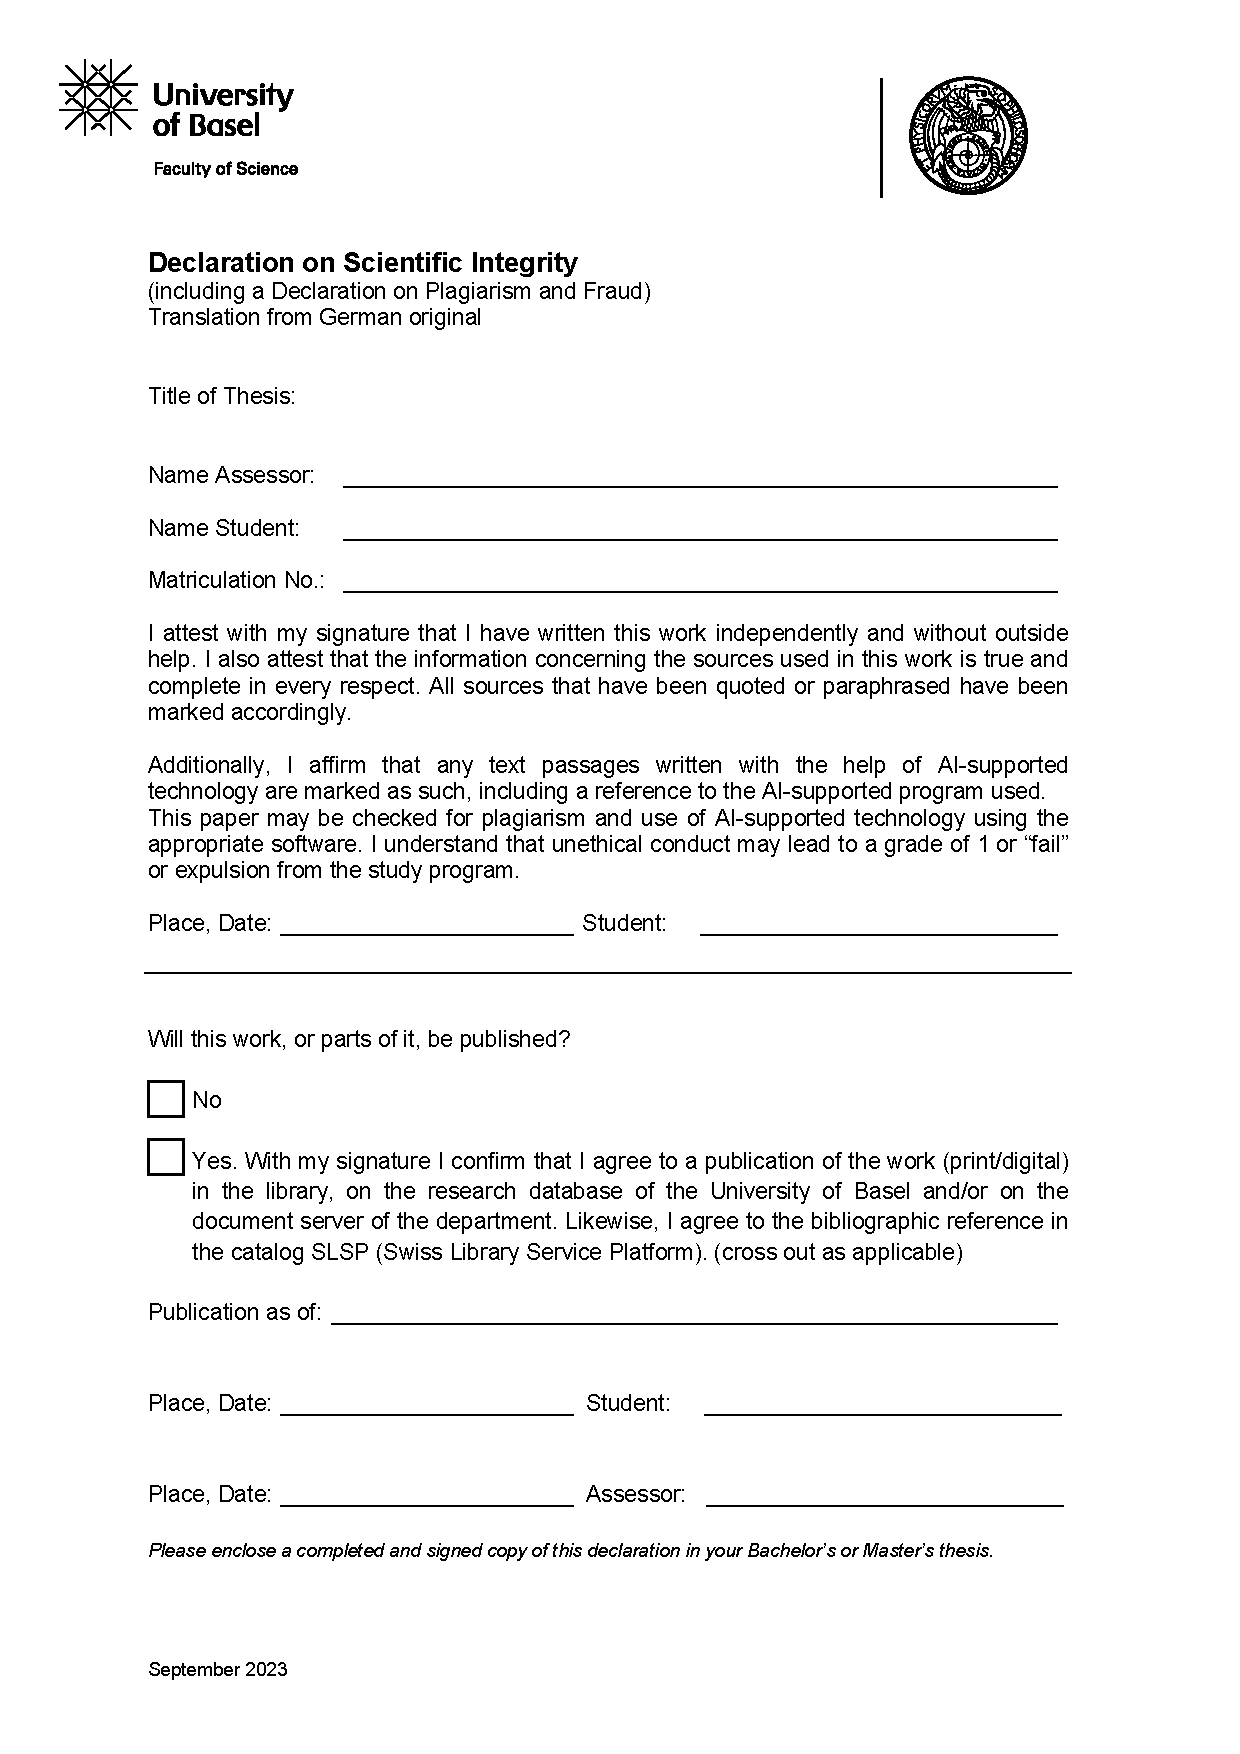
\includepdf{./Back/wissensch_Redlichkeit_E_09-2023.pdf}}
  %{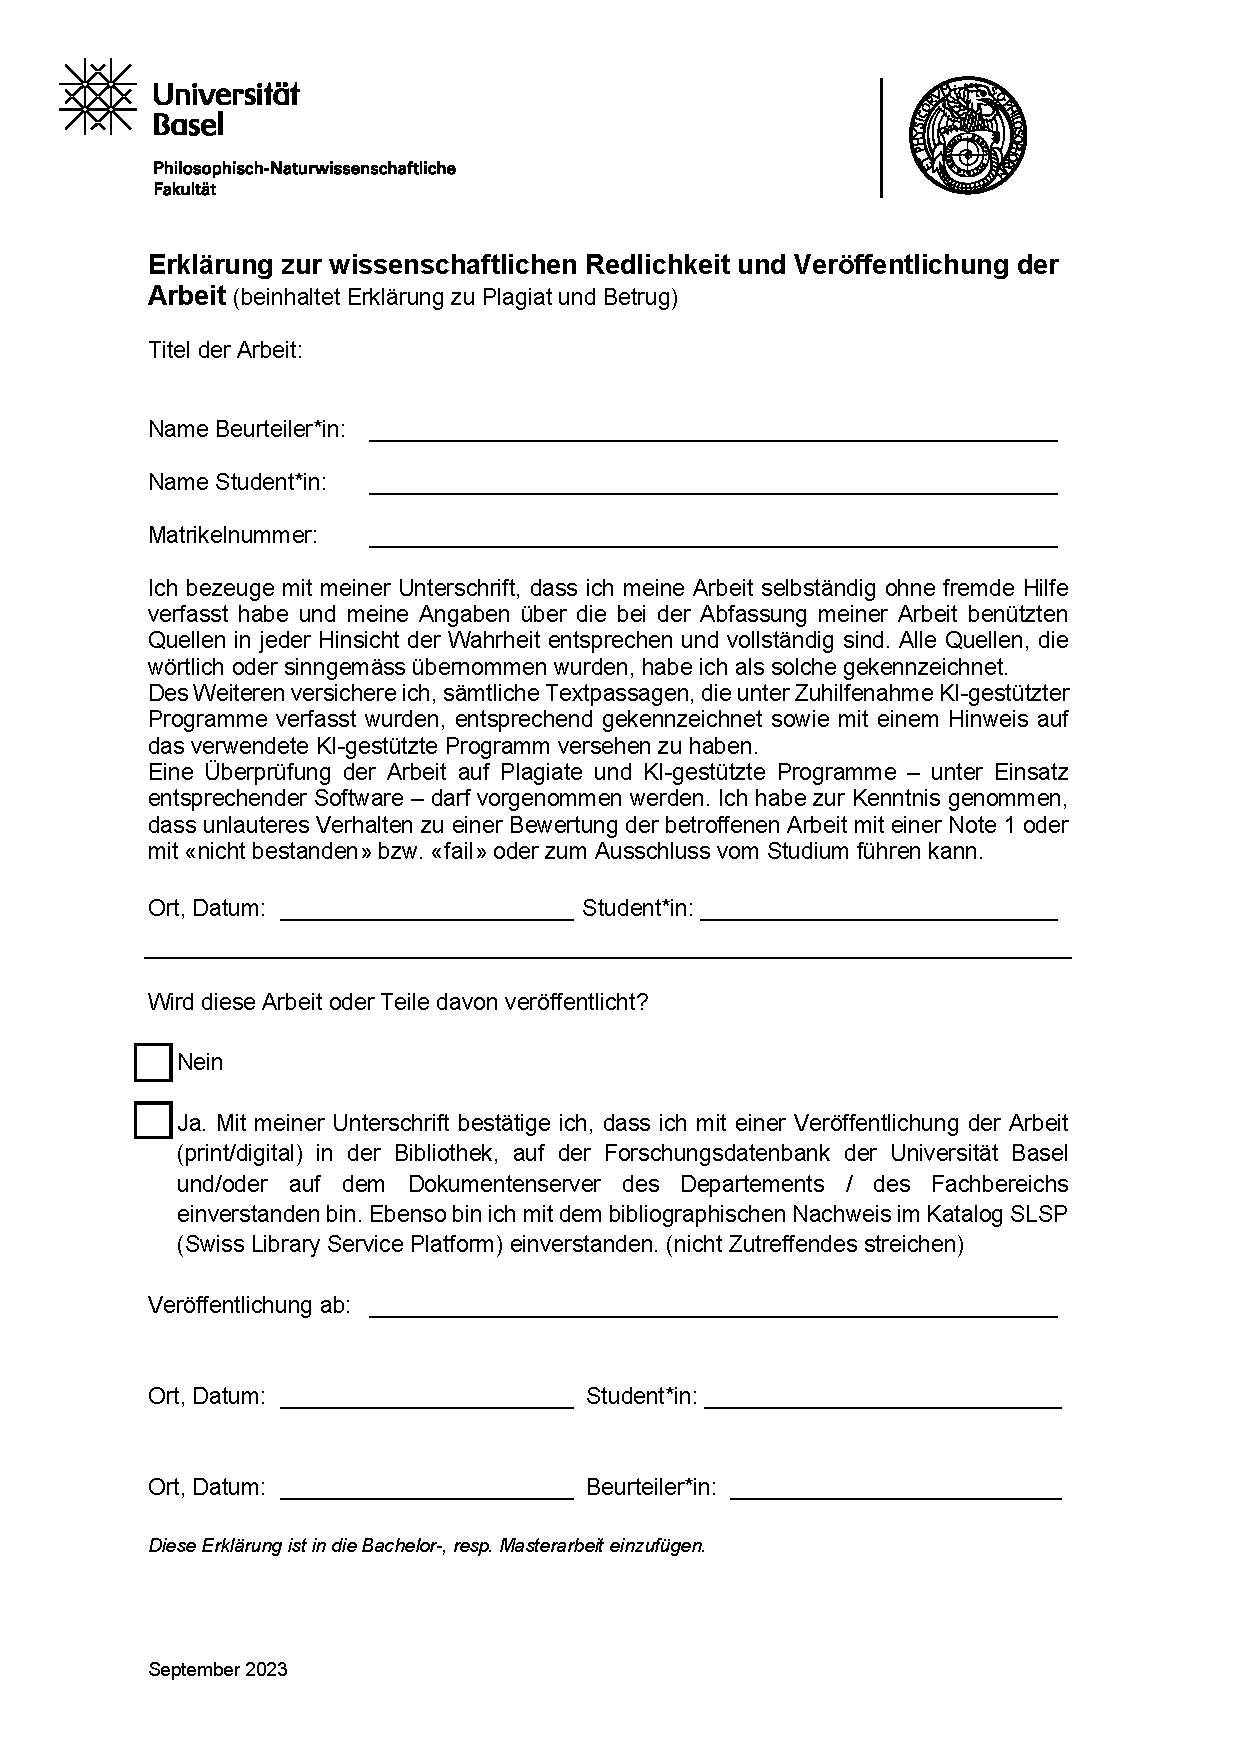
\includepdf{./Back/wissensch_Redlichkeit_D_09-2023.pdf}}
%% ----------------------------------------------------------------
\end{document}
%% ----------------------------------------------------------------
